\documentclass[10pt]{article}

\usepackage[a4paper,margin=1in]{geometry}
\usepackage[T1]{fontenc}
\usepackage[utf8]{inputenc}
\usepackage{amsmath,amssymb}
\usepackage{natbib}
\usepackage{booktabs}
\usepackage{graphicx}
\usepackage{xcolor}
\usepackage{caption}
\usepackage{subcaption}
\usepackage{pgfplots}
\pgfplotsset{compat=1.16}
\usepgfplotslibrary{groupplots}
\usepackage{tikz}
\usetikzlibrary{positioning,arrows.meta,shapes.geometric,calc,fit,backgrounds}
\usepackage[hidelinks]{hyperref}
\usepackage{authblk}

\definecolor{cblue}{HTML}{3A5A8C}
\definecolor{cgreen}{HTML}{4A7A42}
\definecolor{cbrown}{HTML}{8C6D3A}
\definecolor{cred}{HTML}{8C3A3A}
\definecolor{cgrey}{HTML}{8C8C8C}

\captionsetup{font=small,labelfont=bf}
\setlength{\parskip}{2pt}
\setlength{\emergencystretch}{1em}

\title{\bfseries A Self-Correcting World Model for Urban Air-Quality Fields\\[2pt]
on Heterogeneous Low-Cost Sensor Networks}

\author[1]{Melchior Maison}
\affil[1]{\small Canarin Project, Paris, France \quad\texttt{\{firstname.lastname\}@canarin.example}}
\date{October 8, 2026}

% ---- lightweight tikz styles ----
\tikzset{
 blk/.style={rectangle, rounded corners=2pt, draw=cblue!80, fill=cblue!8,
 align=center, inner sep=4pt, minimum height=9mm, font=\footnotesize},
 inp/.style={rectangle, rounded corners=2pt, draw=cbrown!80, fill=cbrown!8,
 align=center, inner sep=3pt, font=\scriptsize},
 onode/.style={rectangle, rounded corners=2pt, draw=cgreen!80, fill=cgreen!8,
 align=center, inner sep=3pt, font=\scriptsize},
 dec/.style={diamond, aspect=2, draw=cbrown!80, fill=cbrown!8, align=center,
 inner sep=1pt, font=\scriptsize},
 res/.style={rectangle, draw=cgrey!80, fill=cgrey!12, align=center,
 inner sep=3pt, font=\scriptsize},
 fl/.style={-{Stealth[length=2.2mm]}, draw=black!65, line width=0.5pt},
 flt/.style={-{Stealth[length=2.2mm]}, draw=cblue!80, line width=1.1pt},
 fld/.style={-{Stealth[length=2.2mm]}, draw=cbrown!80, line width=0.7pt, dashed},
}

\begin{document}
\maketitle

\begin{abstract}
\noindent
Dense networks of low-cost air-quality sensors promise street-level pollution
maps, but their readings are noisy, irregularly sited, and of uncertain
provenance: a device may be broken, indoors, or simply mislocated. We argue that
the pollution field over such a network is best treated as a partially observed
\emph{dynamical system} and modelled with a controller-in-the-loop
\emph{world model} in the sense of Ha and Schmidhuber. Our central design
principle is to factor the problem by \emph{update rate}: near-static context
(building geometry, altitude) conditions the model; exogenous weather acts as the
control input that drives the dynamics; the pollution field is fast latent state;
and per-device properties---reliability, indoor/outdoor exposure, and
position---are slow state that gates how each observation is assimilated. Because
these factors evolve on separate timescales, effects that are otherwise
confounded (a wind-driven plume versus a street-canyon pocket; a faulty sensor
versus a real transient versus a mislocated one) become separable. The controller
does not act on the environment---one cannot steer the air---but on the system's
own trust in each device, an epistemic action space trained in imagination. We
present the architecture, a heterogeneous-device conditioning scheme covering two
sensor classes---an ambient station with onboard GNSS, and a personal-exposure
instrument with none, whose power source governs its mobility, its exposure and
its duty cycle---and runnable components validated against live public data. On a synthetic advective--diurnal
field, a graph-regularized linear baseline attains $53.9\pm4.5\%$ skill over
persistence at a six-hour horizon, establishing a concrete bar that a first
recurrent core, trained on this field, then clears at every horizon beyond one
step---cutting six-hour error by $27\%$ over that baseline, with the mid-horizon
advantage also transferring to real CAMS PM\textsubscript{2.5} measurements. In a
fault-injection study the trust controller down-weights
faulty devices and cuts field-reconstruction error by $13\%$ toward an oracle that
is told which devices have failed; mislocation, catchable only in dense
neighbourhoods, is left to dedicated position state. Because each device reports several
pollutants, we also show that the channel most useful for predicting
particulate mass---humidity, via hygroscopic growth---is almost uncorrelated with
it, so grouping channels by correlation is misleading, and that such covariates
must condition each device's own reading rather than join a shared latent. We release the
design and prototypes as a basis for deployment
on the Canarin network.
\end{abstract}

\section{Introduction}
Low-cost particulate and gas sensors have made it feasible to instrument a city
at the block scale rather than with a handful of reference stations. The
resulting data, however, are hard to use directly. Individual devices drift and
fail; they are placed by volunteers on balconies, indoors, and against building
walls; their reported coordinates may be off by tens of metres. And because the network
is \emph{open}---it accepts readings from any device that can report, from
dedicated boards to phones to third-party hardware---nothing about a contributor's
calibration, siting, or location can be assumed. A naive
interpolation of raw readings inherits every one of these faults, and treating
each sensor independently discards the strong spatial and temporal structure that
makes the data valuable in the first place.

We take the position that the quantity of interest---the ambient pollution
\emph{field}---is a spatiotemporal dynamical system driven by known exogenous
forcing (wind, mixing-layer height, the diurnal cycle) and shaped by static urban
form, and that the sensors are noisy, partially trustworthy observers of it. This
framing invites a \emph{world model}~\citep{ha2018world}: a learned latent
encoder, a recurrent dynamics core that can be rolled forward under hypothetical
forcing, and a controller that closes a feedback loop. The world-model literature
was developed for embodied agents that act to maximize reward. Our setting has no
such lever---Canarin cannot change the air---so we retarget the controller onto
the one thing the system \emph{can} act on: its own beliefs about which sensors to
trust. This is an epistemic, active-inference-flavoured control
problem~\citep{friston2010free}, and it can be trained ``in the dream'' against
the model's own predictions without waiting for real failures.

Our contributions are: (i) an \emph{update-rate factoring} of the problem that
makes otherwise-confounded effects identifiable (\S\ref{sec:setting}); (ii) a
concrete mapping of the encoder/dynamics/controller triple onto a graph encoder,
a stochastic state-space core with weather as the action input, and a
reliability controller, together with a query-conditioned neural-field decoder
for virtual sensors (\S\ref{sec:model}); (iii) a heterogeneous-device conditioning
scheme and an identifiability procedure that disentangles \emph{faulty},
\emph{real-micro-feature}, \emph{indoor}, and \emph{mislocated} explanations of a
disagreeing sensor (\S\ref{sec:model}); and (iv) runnable system components
validated against live public APIs, a multi-seed baseline study that quantifies
the bar the full model must beat, a fault-injection study that empirically
validates the trust controller, and a trained recurrent core---deterministic,
probabilistic, and autoregressive---that clears that bar and whose predictive
bands we calibrate (\S\ref{sec:impl}--\S\ref{sec:rollout}). We are
explicit about scope: the recurrent core is trained on synthetic and real CAMS
data, not on Canarin's own operational readings, which we cannot access from here.

\section{Related Work}
\paragraph{World models and latent dynamics.}
\citet{ha2018world} introduced the vision-model / memory-RNN / controller
decomposition; latent state-space variants such as
PlaNet~\citep{hafner2019planet} and Dreamer~\citep{hafner2020dream} showed that a
stochastic recurrent core supports planning and control entirely in latent space.
We borrow this decomposition but replace pixel frames with an irregular sensor
graph and replace agent actions with meteorological forcing.

\paragraph{Spatiotemporal forecasting.}
Graph neural networks with recurrent or diffusion structure are standard for
sensor-network forecasting~\citep{kipf2017gcn,li2018dcrnn}. Such models typically
assume trustworthy, correctly located nodes; our contribution is orthogonal and
complementary: a mechanism for deciding \emph{how much each node should count}.

\paragraph{Continuous decoders.}
Coordinate-based neural fields~\citep{mildenhall2020nerf,sitzmann2020siren} map a
location to a value, enabling queries at arbitrary points. We use a
field decoder to read the latent state at unmonitored locations (``virtual
sensors'').

\paragraph{Data assimilation.}
Sequentially correcting a dynamical state against noisy observations with an
uncertainty budget is classical data assimilation; the ensemble Kalman
filter~\citep{evensen2003enkf} is the canonical example. Our recurrent posterior
update plays the same role, with the controller adjusting the observation-error
covariance per device.

\paragraph{Low-cost air quality.}
The promise and pitfalls of low-cost sensing are well
documented~\citep{lewis2016validate,zheng2013uair}; calibration drift and siting
are the dominant error sources, motivating our explicit per-device reliability and
exposure state. Urban canopy parameters such as street-canyon aspect ratio and
sky-view factor are standard descriptors of dispersion
geometry~\citep{oke1988street}.

\section{Problem Setting and Design Principles}
\label{sec:setting}
A Canarin device is not a single-species instrument, and its channels are not all
of the same kind. A Pico carries a Plantower PMSA003 particulate counter
(three size bins), a Sensirion SGP40 gas sensor (a VOC index plus derived and raw
signals), and Bosch BME280 and BME680 environmental sensors---so a single unit
reports a dozen or so distinct \texttt{normalized\_code}s, of at least four
different semantic types (Table~\ref{tab:channels}). Throughout the paper
\texttt{normalized\_code} is the canonical pollutant identity; in the deployed
platform it is \texttt{WebFront.pollutant\_types.id}, reached through each
device's channel declaration in \texttt{WebFront.pollutants}
(\S\ref{sec:birdhouse}). Treating them as
interchangeable ``pollutants'' would be a modelling error: only some are ambient
field quantities at all.

Three distinctions are load-bearing. First, \emph{a value's role is not its
units}. The particulate bins are ambient concentrations to be mapped and
forecast; the VOC index is a bounded ordinal index, not a concentration; raw
$\mathrm{H_2}$/ethanol signals and gas resistance are instrument-internal
diagnostics; and pressure and humidity are ambient covariates that condition the
interpretation of the others---optical particulate counts inflate at high humidity
through hygroscopic growth. Second, and easy to get wrong: \textbf{the temperature
channel measures the device's own heat, not ambient air temperature.} It is a
housekeeping and calibration covariate; the device cannot sense ambient
temperature at all, which is precisely why the platform obtains it from the
external weather service (\S\ref{sec:impl}) rather than from the fleet. Third,
some channels are \emph{duplicated within one device}---BME280 and BME680 both
report pressure and humidity---which the \texttt{instance\_index} disambiguates
and which, as \S\ref{sec:multi} notes, provides a free intra-device consistency
check.

\paragraph{Four blocks, one of them open.}
The model reads from Plumage, which stores every observation as a tuple
\begin{equation}
\big(\texttt{device\_id},\ \texttt{instance\_index},\ \texttt{normalized\_code},\
\texttt{ts},\ \texttt{value}\big),
\label{eq:tuple}
\end{equation}
so a record is recovered by grouping on $(\texttt{device\_id},\texttt{ts})$. The
codes in a record do not form one homogeneous vector: they fall into four blocks
whose \emph{arity stability} differs, and that difference---not the physics---is
what should drive the architecture (Table~\ref{tab:blocks}). Three blocks have
fixed, known width: \textsc{geo} (latitude, longitude, and a quality covariate),
\textsc{hardware} (battery state and board temperature), and \textsc{weather}
(delivered by the weather service, which shares the normalized-code vocabulary but
is keyed by grid cell and hour rather than by device---see below). Only
the fourth, \textsc{sensing}---pollutants and whatever else a contributor
reports---is an open set that grows over the life of the deployment.

Two consequences follow, and they simplify rather than complicate the design.
First, \emph{only \textsc{sensing} needs dynamic handling}; the other three use
ordinary fixed-width encoders, so the complexity is confined to one block instead
of infecting the whole input path. Second, the split lines up with the update-rate
factoring of Table~\ref{tab:tiers}: \textsc{geo} is near-static for a Pico and fast
for a phone-powered Femto, \textsc{hardware} is slow, \textsc{weather} is the exogenous
fast input $u_t$, and \textsc{sensing} is the fast state being modelled. The blocks
are therefore not an implementation convenience but the same seam the model is
already built around.

A constraint attaches to \textsc{hardware}: it must reach the trust controller and
the observation model, never the field decoder. Battery level and board
temperature are evidence about the \emph{instrument}---a sagging battery precedes
brownout, a hot board biases the collocated humidity and gas channels---and letting
them predict concentrations would let the model learn ``this hardware reads high,''
the identical leakage the paper forbids for device type.

\paragraph{The types table carries the block.}
Block membership is a property of a \emph{code}, not something the model should
infer from the code's spelling. Murmuration therefore keeps a type registry
(\texttt{Murmuration.type\_registry}, keyed by pollutant type) with the block and the finer role
(\texttt{block} $\in$ \{geo, hardware, weather, sensing\}; \texttt{role} $\in$
\{target, covariate, diagnostic, derived, housekeeping, exogenous\}), together with
the flags the model needs: whether a code gets a decoder head, whether it may join
a tranche, its cold-start trust prior, its ingestion sanity window, and---for
nested quantities---a \texttt{parent\_code} and constraint kind. Enrolling a new
sensor is then a row insert, not a code change, and the model derives its whole
plan for a cycle from that table: which codes to decode, which to condition on,
which pairs to gate, which are eligible for tranche assignment. The consistency
gates in particular fall out of the data rather than being hardcoded---declaring
$\texttt{pm1}\rightarrow\texttt{pm25}\rightarrow\texttt{pm10}$ with
\texttt{le\_parent} is what generates the checks of \S\ref{sec:multi}. An
unregistered code degrades safely: it lands in \textsc{sensing}, receives no
decoder head and a low trust prior, and contributes nothing until it is described.

\paragraph{Weather is stored once per cell-hour, not once per device.}
An earlier version of this design wrote the resolved weather back under each
device's own key. That is simple to read but wrong in one important respect: the
model maintains a position correction $\Delta p$, so a device's location can be
revised after the fact, at which point per-device weather rows are attached to the
wrong cell and must all be rewritten. We instead store weather once per
$(\texttt{cell\_id}, \texttt{ts\_hour})$ and stamp each reading with the
\texttt{cell\_id} that was resolved for it---one integer per record rather than a
set of float rows. This keeps the read-side join a plain key lookup, cuts weather
storage by a further factor of twenty on the fleet of Table~\ref{tab:wx}, lets a
position correction re-resolve cleanly, and---because the cell is recorded rather
than recomputed---preserves the provenance needed to answer what the model actually
saw, even if the grid resolution or provider later changes.

\paragraph{Tranches within the open block.}
Because \textsc{sensing} alone varies, only it is split into \emph{tranches}: small
cores each covering a few codes, spawned and retired by a registry as codes appear
and disappear, versioned and rolled back independently, and combined by fusing
their \emph{residuals} rather than their outputs (\S\ref{sec:multi}). Membership is
decided by measured \emph{predictive gain}---does one code's history improve the
forecast of another beyond its own history---and emphatically not by correlation,
which we find points the wrong way (\S\ref{sec:multi}). A new code enters as a
singleton tranche with near-zero trust, and is merged once enough history exists to
measure whether it belongs anywhere, which is also when its credibility score
(\S\ref{sec:credibility}) first becomes meaningful.

\begin{table}[t]
\centering
\small
\begin{tabular}{@{}llll@{}}
\toprule
Block & Contents & Arity & Role \\
\midrule
\textsc{geo} & lat, lon (+ fix quality) & fixed & spatial weighting, position state \\
\textsc{hardware} & battery, board temperature & fixed & health/trust; \emph{never} the field \\
\textsc{weather} & from weather service, keyed (cell, hour) & fixed & control input $u_t$ \\
\textsc{sensing} & pollutants and others & \textbf{variable} & fast state $\rightarrow$ \textbf{tranches} \\
\bottomrule
\end{tabular}
\caption{The four blocks of a record, joined by
$(\texttt{device\_id},\texttt{ts})$. Only \textsc{sensing} has variable width, so
only it requires dynamic handling; the split coincides with the update-rate tiers
of Table~\ref{tab:tiers}.}
\label{tab:blocks}
\end{table}

We seek a latent field state $z_t$ whose decoder $g(\cdot)$ predicts, at
\emph{any} location, each channel designated as an ambient target; a short-horizon
rollout $z_{t+1{:}t+h}$ under a weather forecast; calibrated uncertainty; and a
per-device trust weight. Trust is per \emph{channel} as well as per device: a unit
whose particulate counter has failed may still report humidity correctly, and
amputating the whole device would discard good data.

\begin{table}[t]
\centering
\small
\begin{tabular}{@{}llll@{}}
\toprule
Sensor & Channels & Semantic type & Role in the model \\
\midrule
Plantower PMSA003 & PM\textsubscript{1}, PM\textsubscript{2.5}, PM\textsubscript{10}
 & mass concentration & \textbf{ambient target} \\
Sensirion SGP40 & VOC index & bounded index (0--500) & ambient target (ordinal) \\
 & eCO\textsubscript{2} & \emph{derived} estimate & derived, not measured \\
 & rawH\textsubscript{2}, rawEthanol & raw sensor signal & diagnostic / calibration \\
BME680 & gas resistance & raw sensor signal & diagnostic / calibration \\
BME280, BME680 & pressure, humidity & ambient physical & \textbf{covariate} (duplicated) \\
BME680 & temperature & \emph{device self-heat} & \textbf{housekeeping}, not ambient \\
\midrule
Weather service & ambient temp., wind, \dots & external, per cell-hour & control input $u_t$ \\
\bottomrule
\end{tabular}
\caption{Channels reported by a Canarin Pico, by semantic type. Only the first
group are ambient quantities to be mapped; the temperature channel reads the
device's own heat and is never treated as ambient air temperature, which the
platform takes from the weather service instead. Pressure and humidity appear
twice per device, on two different sensors.}
\label{tab:channels}
\end{table}

\paragraph{Factor by update rate.}
The influences on $y_{i,t,c}$ change on very different timescales, and building the
model around that seam is what makes them separable (Table~\ref{tab:tiers}).
Corridors and heat pockets \emph{emerge} from the interaction of a fast term
(wind) and a slow term (geometry). Because wind varies while geometry does not,
the two can be disentangled from observations alone: geometry is invariant across
wind conditions, whereas the wind effect co-varies with wind. The same logic
later separates a faulty sensor (a persistent signature) from a real transient
(co-varying with conditions) and from a mislocated sensor (a residual explained by
a spatial shift).

\begin{table}[t]
\centering
\small
\begin{tabular}{@{}llll@{}}
\toprule
\textbf{Tier} & \textbf{Quantity} & \textbf{Update rate} & \textbf{Role} \\
\midrule
Static context & altitude, canyon geometry, land use & $\sim$never & conditioning \\
Exogenous & wind, temperature, mixing height & every step & control input $u_t$ \\
Fast state & pollution field latent $z_t$ & every step & evolved, assimilated \\
Slow state & reliability, exposure, position & hours--days & gate observations \\
Attribute & device type & fixed & selects obs./location model \\
\bottomrule
\end{tabular}
\caption{Update-rate factoring of the problem. Separating quantities by how fast
they change is the load-bearing design choice: it renders confounded effects
identifiable.}
\label{tab:tiers}
\end{table}

\section{Model}
\label{sec:model}
We instantiate the world-model triple as an encoder $V$, a dynamics core $M$, and
a controller $C$, with a separate neural-field decoder $g$ (Fig.~\ref{fig:arch}).

\begin{figure}[t]
\centering
\resizebox{\linewidth}{!}{%
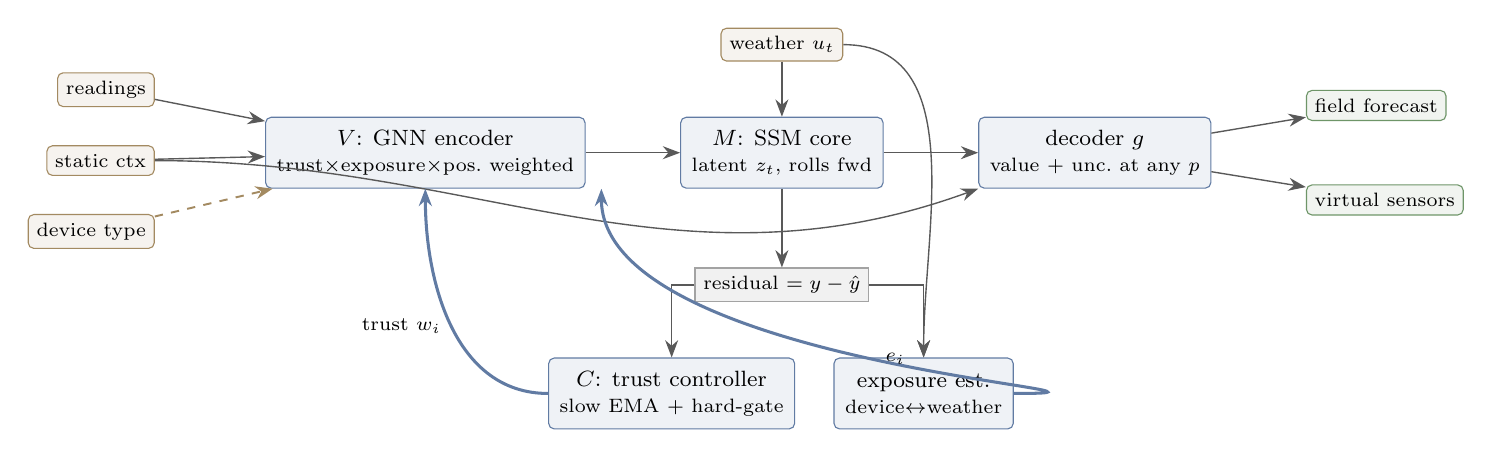
\begin{tikzpicture}[node distance=8mm and 12mm]
 % core
 \node[blk] (V) {$V$: GNN encoder\\\scriptsize trust$\times$exposure$\times$pos.\ weighted};
 \node[blk, right=of V] (M) {$M$: SSM core\\\scriptsize latent $z_t$, rolls fwd};
 \node[blk, right=of M] (G) {decoder $g$\\\scriptsize value + unc.\ at any $p$};
 % inputs (left)
 \node[inp, left=14mm of V, yshift=8mm] (R) {readings};
 \node[inp, left=14mm of V, yshift=-1mm] (ST) {static ctx};
 \node[inp, left=14mm of V, yshift=-10mm] (DT) {device type};
 % weather on top of M
 \node[inp, above=7mm of M] (WX) {weather $u_t$};
 % controller + exposure (below)
 \node[res, below=10mm of M] (RES) {residual $= y-\hat y$};
 \node[blk, below=7mm of RES, xshift=-14mm] (C) {$C$: trust controller\\\scriptsize slow EMA + hard-gate};
 \node[blk, below=7mm of RES, xshift=18mm] (E) {exposure est.\\\scriptsize device$\leftrightarrow$weather};
 % outputs
 \node[onode, right=12mm of G, yshift=6mm] (FF) {field forecast};
 \node[onode, right=12mm of G, yshift=-6mm] (VS) {virtual sensors};

 \draw[fl] (R) -- (V); \draw[fl] (ST) -- (V);
 \draw[fld] (DT) -- (V);
 \draw[fl] (ST.east) to[out=0,in=200] (G.south west);
 \draw[fl] (WX) -- (M);
 \draw[fl] (V) -- (M); \draw[fl] (M) -- (G);
 \draw[fl] (G) -- (FF); \draw[fl] (G) -- (VS);
 \draw[fl] (M) -- (RES); \draw[fl] (RES) -| (C);
 \draw[fl] (RES) -| (E);
 \draw[fl] (WX.east) to[out=0,in=90] (E.north);
 \draw[flt] (C.west) to[out=180,in=270] node[midway,left,font=\scriptsize]{trust $w_i$} (V.south);
 \draw[flt] (E.east) to[out=0,in=270] node[midway,right,font=\scriptsize]{$e_i$} ($(V.south east)+(2mm,0)$);
\end{tikzpicture}%
}
\caption{Architecture. Solid arrows carry data and feedback; the dashed arrow is
\emph{conditioning}: device type parameterizes the observation/location model
rather than supplying a field value. Weather enters $M$ as the control input
$u_t$. The controller $C$ and the exposure estimator produce slow per-device
state that re-weights assimilation in $V$, closing the loop.}
\label{fig:arch}
\end{figure}

\paragraph{Encoder $V$.}
A graph neural network over the irregular sensor graph maps the current
observation batch, static context, and weather to the field latent $z_t$. Each
reading enters with weight proportional to $w_i\cdot e_i\cdot c_i$---trust,
exposure, and position-confidence---so that broken, indoor, or poorly located
devices influence the field less without being discarded.

\paragraph{Dynamics core $M$.}
A stochastic state-space core (an RSSM-lite recurrence) propagates $z_t\to
z_{t+1}$ with the weather forecast occupying the \emph{action} slot of the
classic memory RNN. Rolling the core forward under a forecast yields the
multi-step field prediction; assimilating the next real batch is the posterior
update of the state-space filter and supplies uncertainty bands, whose realized
calibration we probe in \S\ref{sec:calibcore}.

\paragraph{Decoder $g$.}
A coordinate-conditioned neural field reads $z_t$ at any $(lat,lon)$, producing
both real-sensor reconstructions and virtual-sensor estimates with uncertainty.
Keeping encode and decode separate is what enables queries away from device
locations.

\paragraph{Controller $C$.}
Because there is no environmental action, $C$ acts on the observation model
itself: it maintains a per-device trust weight $w_i$ that enters $V$'s
assimilation gain. Trust evolves as a slow, asymmetric exponential moving average
of agreement,
\begin{equation}
w_i \leftarrow w_i + \eta\,(a_{i,t}-w_i), \qquad \eta \text{ small}, \quad
\eta^{-}>\eta^{+},
\label{eq:trust}
\end{equation}
where $a_{i,t}$ is the agreement between the device and its expected reading, and
the asymmetry makes trust easier to lose than to regain. An unambiguous fault
(flatline, dropout, rail-pinned value) bypasses the EMA through a hard gate, while
a periodic \emph{forced-listening} probe re-admits a distrusted device at full
weight to test whether it has recovered. Trust can be trained against the model's
own imagined rollouts, so failures need not be observed in the wild first.

\paragraph{Multiple channels per device.}
Because each device reports a dozen typed channels, the encoder consumes the
\emph{set} $\mathcal{O}_t$ of Eq.~\eqref{eq:tuple} through per-code embeddings and
per-code standardization---channels differ by orders of magnitude and in kind, so a
single scaler is meaningless across a VOC index and a pressure in hPa. Decoder
heads are emitted only for channels designated as ambient targets. Three design
points follow. (i)~\emph{Cross-channel coupling is real signal}: the three
particulate bins are nested size fractions and move together, humidity drives
apparent particulate mass through hygroscopic growth, and the VOC index responds to
the same combustion sources as the fine fraction. A model that sees the set can use
one channel to predict another. (ii)~\emph{Cross-channel physics gives
density-independent fault gates.} Two hold on a single device with no neighbour at
all: the nested-fraction inequality
$\text{PM}_{1}\!\le\!\text{PM}_{2.5}\!\le\!\text{PM}_{10}$, which the Plantower's
three bins make checkable directly; and the \emph{duplicate-sensor} agreement
between the BME280 and BME680 pressure and humidity channels on the same board,
which should track within tolerance and whose divergence localizes the failure to
one of the two sensors. This matters precisely where the trust loop is weakest
(\S\ref{sec:faults}): spatial disagreement needs neighbours and collapses on sparse
networks, whereas these gates read one device's own channels.
(iii)~\emph{Role, not units, decides use}: pressure and humidity condition the
observation model; raw $\mathrm{H_2}$, raw ethanol and gas resistance feed
calibration and health, not the field; eCO\textsubscript{2} is a derived estimate
rather than a measurement and is never treated as ground truth; and the temperature
channel, being device self-heat, is a health covariate whose \emph{rise} is itself
a fault signature---a hot board biases the collocated humidity and gas readings.

\paragraph{Sharing capacity across channels.}
Whether one core should model all channels jointly is an empirical question, not a
matter of taste, and \S\ref{sec:multi} answers it on the device's real
channels: every way of merging them into one flat state degrades the targets, so
the core is factored into tranches over targets while covariates enter through
per-device conditioning. The block decomposition of \S\ref{sec:setting} is what
keeps that arrangement stable as new codes arrive.

\paragraph{Per-device slow state and conditioning.}
Three properties are learned per device and one is declared. \emph{Reliability}
answers whether the device works; \emph{exposure} answers whether it samples the
outdoor field at all, learned as the strength of the device--weather coupling and
best represented as a continuous coefficient that doubles as the assimilation
weight; \emph{position} is treated uncertainty-first---a shaky fix informs the
field over a blurred location before any correction---with an optional,
tightly-constrained $\Delta p$ correction that exploits the decoder's
differentiability in query location. \emph{Device type} is a known attribute that
parameterizes the observation and location-error model and seeds cold-start priors
(Table~\ref{tab:devtype}); crucially it conditions the \emph{interpretation} of a
reading, never the field value directly, so the model cannot learn a spurious
``type $X$ reads higher'' shortcut.

\begin{table}[t]
\centering
\small
\begin{tabular}{@{}lll@{}}
\toprule
& \textbf{Pico} & \textbf{Femto} \\
& \emph{ambient station} & \emph{personal medical instrument} \\
\midrule
Hardware & LilyGO-class board + u-blox GNSS & own MCU, no GNSS \\
Power source & mains or battery & \textbf{host phone, or mains} \\
Connectivity & cellular or Wi-Fi (UDP) & via host phone, or own Wi-Fi \\
Location source & onboard GNSS & phone GPS, Wi-Fi positioning, or declared \\
Indoor fix & no (blind) & yes (non-GNSS) \\
Position error & multipath, sidereal-repeatable & tens to hundreds of metres \\
Quality covariate & HDOP, satellite count & \texttt{position\_source}, accuracy radius \\
Duty cycle & continuous & \textbf{gated by its power source} \\
What it samples & the \textbf{ambient field} & the \textbf{carrier's exposure} \\
Role in assimilation & full weight & reduced or none when phone-powered \\
\bottomrule
\end{tabular}
\caption{Device archetypes. The classes differ in kind, not merely in error
regime. A Pico is an ambient station; a Femto is a medical instrument measuring a
person's exposure, with no satellite receiver in either mode. Its power source is
the governing variable---phone-powered implies carried, mobile and personal;
mains-powered implies plugged in, static and almost certainly indoors---and
connectivity, location and duty cycle all follow from it. Device type therefore
selects the position prior, the exposure prior \emph{and} the assimilation weight,
without ever acting as a feature of the field itself. The fleet remains
\emph{open}: any device able to emit the wire format may contribute, so these are
archetypes rather than an exhaustive list.}
\label{tab:devtype}
\end{table}

\paragraph{Power source is the governing covariate, and exposure is not a fault.}
Two consequences follow from a device whose operation is gated by what powers it.
First, \emph{absence is not unreliability}. A phone-powered Femto stops when the
phone is off, out of range or unplugged; the resulting gaps are duty cycle, not
failure, and the trust controller must not penalize them. The credibility score
counts effective fleet size by timeliness rather than enrolment
(\S\ref{sec:credibility}), which is correct here for a benign reason: such a
device genuinely supports the live field only part of the time, while remaining
sound.

Second, and more consequential for the architecture, \emph{low outdoor coupling is
the product rather than a defect}. Elsewhere in this paper a device decoupled from
the ambient field is an \emph{indoor fault} to be down-weighted
(\S\ref{sec:faults}). For a Femto measuring a patient's exposure it is the
measurement. A mains-powered Femto is plugged into a wall socket and therefore
almost certainly indoors; a phone-powered one follows its carrier through vehicles,
offices and other people's homes. Neither is evidence about outdoor air at its
reported coordinates. The system therefore serves two products from one pipeline:
Pico readings assimilate into the ambient field at full weight, while Femto
readings carry the personal-exposure product at full value and enter the ambient
field at reduced weight or not at all. The exposure estimator is seeded from the
declared power source instead of having to infer it from residuals over days.

\paragraph{Reliability across the device hierarchy.}
Reliability need not be estimated per instance in isolation. Canarin devices form a
natural hierarchy---\emph{type} (Pico / Femto) over \emph{device model} (a specific
board or sensor revision) over \emph{instance}---and reliability, together with the
location-error scale, is partially pooled up this hierarchy: each instance's trust
prior is drawn from its device model's distribution, and each device model's from
its type's. Three consequences follow. (i)~\emph{Cold start}: a freshly enrolled
unit inherits its device model's prior rather than a flat one, so a new instance of
a known-good model is trusted sooner and one of a known-flaky model is treated with
caution. (ii)~\emph{Systematic-defect detection}: a fault shared by most instances
of a device model shifts the \emph{device-model-level} parameter, which is
distinguishable from an instance-level failure---the difference between ``this unit
is broken'' and ``this revision is biased.'' (iii)~\emph{Procurement signal}: the
device-model-level posterior ranks revisions by field reliability, informing which
hardware to deploy. This is a standard partial-pooling (random-effects) structure
over the per-device trust state; it is specified here and left for training on
operational data.

\paragraph{Identifiability: which twin?}
A device's \emph{twin} is the model's expectation of its reading; exposure selects
which twin it is judged against. A disagreement with the outdoor-field twin then
has four possible causes, resolved in sequence (Fig.~\ref{fig:twin}): a small
position shift (mislocated), the static context (a real micro-feature such as a
canyon pocket), temporal persistence (a fault), or none of these (a genuine
transient, and an alert candidate). Reliability and exposure are orthogonal axes,
so the system never ``repairs'' a healthy indoor sensor.

\begin{figure}[t]
\centering
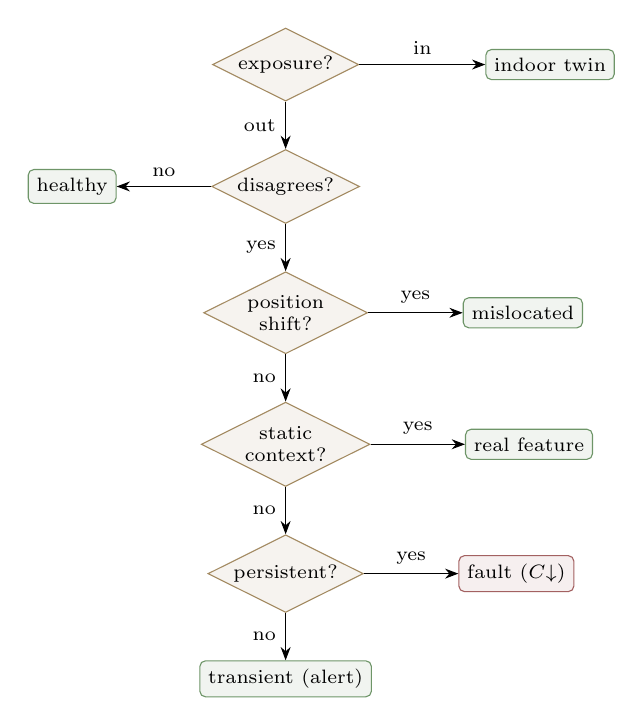
\begin{tikzpicture}[node distance=6mm and 10mm, >=Stealth]
 \node[dec] (exp) {exposure?};
 \node[onode, right=16mm of exp] (indoor) {indoor twin};
 \node[dec, below=of exp] (dis) {disagrees?};
 \node[onode, left=12mm of dis] (ok) {healthy};
 \node[dec, below=of dis] (pos) {position\\shift?};
 \node[onode, right=12mm of pos] (mis) {mislocated};
 \node[dec, below=of pos] (sc) {static\\context?};
 \node[onode, right=12mm of sc] (real) {real feature};
 \node[dec, below=of sc] (per) {persistent?};
 \node[rectangle,rounded corners=2pt,draw=cred!80,fill=cred!8,inner sep=3pt,
 font=\scriptsize, right=12mm of per] (fault) {fault ($C{\downarrow}$)};
 \node[onode, below=of per] (trans) {transient (alert)};

 \draw[->] (exp) -- node[above,font=\scriptsize]{in} (indoor);
 \draw[->] (exp) -- node[left,font=\scriptsize]{out} (dis);
 \draw[->] (dis) -- node[above,font=\scriptsize]{no} (ok);
 \draw[->] (dis) -- node[left,font=\scriptsize]{yes} (pos);
 \draw[->] (pos) -- node[above,font=\scriptsize]{yes} (mis);
 \draw[->] (pos) -- node[left,font=\scriptsize]{no} (sc);
 \draw[->] (sc) -- node[above,font=\scriptsize]{yes} (real);
 \draw[->] (sc) -- node[left,font=\scriptsize]{no} (per);
 \draw[->] (per) -- node[above,font=\scriptsize]{yes} (fault);
 \draw[->] (per) -- node[left,font=\scriptsize]{no} (trans);
\end{tikzpicture}
\caption{Resolving a disagreeing sensor. Static context, exposure, and position
each absorb one benign explanation; only what survives all three is treated as a
fault, and only a non-persistent survivor becomes an alert.}
\label{fig:twin}
\end{figure}

\paragraph{Inference loop.}
Each cycle (Algorithm-style summary): (1) read and normalize the batch; (2) encode
with weights $w_i e_i c_i$ and the type-selected observation model; (3) roll $M$
forward under the weather forecast and decode to real and virtual points; (4)
assimilate the next batch, forming residuals against each twin; (5) update the
slow state---trust via Eq.~\eqref{eq:trust}, exposure from device--weather
coupling, position under its constraints; (6) write field forecasts, uncertainty
bands, virtual sensors, anomaly scores, trust, exposure, and position to the
store.

\section{System Implementation}
\label{sec:impl}
The model is not a standalone research artifact but a service embedded in the
operational Canarin stack on AWS (one ECS Fargate cluster, an RDS MySQL~8.4
instance holding the schemas \texttt{Data}, \texttt{Devices}, \texttt{WebFront}
and \texttt{Users}, and an ElastiCache Redis node). In that stack, ingestion is
handled by \emph{Birdhouse}, the authoritative store and dashboard by
\emph{Plumage}, alerting by \emph{Chirping}, and ambient weather by
\emph{Thermal}; the world model runs as a separate service we call
\emph{Murmuration}. We describe the ingestion protocol and data model the model
inherits, the two feature services, and---in detail---how Murmuration reads from
and writes to the platform stores. This section describes the platform as
deployed (October 2026, Murmuration v0.1); where the design goes beyond what is
deployed we say so.

\subsection{Ingestion protocol and data model (Birdhouse)}
\label{sec:birdhouse}
Canarin devices connect over cellular \emph{or} Wi-Fi and typically sit behind
carrier-grade or home NAT; they cannot be addressed inbound and therefore initiate
every connection outbound, with bidirectional control over a cellular link
requiring a private APN. Telemetry is emitted as compact \textbf{UDP} datagrams,
which suit lossy, bandwidth-constrained links and keep the device firmware trivial.
The wire protocol is deliberately \emph{open}: any device able to emit a normalized
datagram---a dedicated Canarin board, a smartphone, or third-party hardware---can
contribute to the collection, which is exactly why the platform assumes nothing
about a contributor and estimates trust, exposure, and position per device. The
ingestion tier scales horizontally without a coordinator: multiple socket workers
share one port via \texttt{SO\_REUSEPORT} behind a network load balancer on ECS
Fargate, so throughput grows with worker count.

Two invariants are established \emph{at ingestion}, before any storage, and the
rest of the platform---the model included---relies on them:
\begin{itemize}\itemsep1pt \topsep2pt
\item \textbf{Unit normalization.} Each raw channel value is scaled by a
per-pollutant \texttt{scale\_factor} into canonical units, so magnitudes are
comparable across device revisions and sensor vendors.
\item \textbf{Identity normalization.} Each value is resolved to a
\emph{channel declaration}: a row of \texttt{WebFront.pollutants} keyed by
(\texttt{device\_id}, \texttt{pollutant\_type\_id}, \texttt{granularity},
\texttt{instance\_index}) that names the canonical pollutant type
(\texttt{WebFront.pollutant\_types}: PM1, PM2.5, PM10, TVOC, CO2, humidity,
pressure, temperature, battery, \ldots), carries the \texttt{scale\_factor}, and
maps the legacy per-device \texttt{value\_id} the firmware still emits. Channels
without a declaration are quarantined (\texttt{Data.data\_points\_quarantine})
rather than stored under a guessed identity---the ``unregistered code degrades
safely'' rule of \S\ref{sec:setting} is enforced one step earlier than the
model. A composite primary key on (\texttt{device\_id},
\texttt{time\_bucket}, \texttt{pollutant\_id}) in
\texttt{Data.data\_points\_canonical} makes each observation a single,
idempotent row; the timestamp is bucketed to the channel's granularity.
\end{itemize}
The hot path performs only enrichment---an in-process, MySQL-backed cache of the
channel declarations (five-minute TTL)---then does two things: it writes the
canonical record to the authoritative store and \emph{fans it out} by appending
one entry to a Redis stream (\texttt{birdhouse:fanout}) on the shared ElastiCache
node. The entry carries the device, the channel, the bucketed event time, the
canonical value, and the server's arrival time; the append is bounded in length
and any Redis error is logged and swallowed. \textbf{Nothing model-related runs
on this path}; Murmuration reads the stream with its own consumer group, strictly
downstream, so inference latency can never back-pressure ingestion, and a
consumer that is down simply resynchronizes from the store when it returns.

\subsection{Feature services: weather and static context}
\label{sec:thermal}
\emph{Thermal} is the design for the weather feature service; in the deployed
platform ambient weather is fetched by Plumage's \texttt{Ambient} service
(Open-Meteo or M\'et\'eo-France providers) for display, and it is not yet wired
into Murmuration as the control input $u_t$---v0.1 runs the kriging encoder of
\S\ref{sec:deployed} without exogenous forcing. The rest of this subsection
describes the service as designed and prototyped. Thermal resolves ambient
weather per site from a public provider,
decomposes wind into $(u,v)$ components---interpolation on a direction
\emph{angle} across the $0/360^\circ$ wrap is incorrect---and interpolates the
hourly forecast to the nowcast cadence; on provider failure it serves the last
good value flagged stale and the model widens its uncertainty. Ambient weather is
kept strictly distinct from a device's \emph{internal} temperature, which is a
calibration and health covariate and, on Canarin hardware, the only temperature the
device itself can report.

\paragraph{Attaching weather to every transmission.}
The weather block is defined per record, so Thermal enriches \emph{each
transmission}: it takes the reporting device's position and timestamp, resolves the
ambient conditions there and then, and writes them back into Plumage under the same
composite key as the sensor rows. The read path is then a plain join on
$(\texttt{device\_id},\texttt{ts})$ with no special-casing, which is what makes
\textsc{weather} an ordinary fixed-width block rather than a bespoke pathway.

Done naively---one provider request per transmission, one stored row per
transmission---this does not survive contact with an open fleet, for three reasons,
each with a corresponding measure (Table~\ref{tab:wx}).
\emph{Volume}: thirty devices at twelve transmissions an hour is $60{,}480$ requests
a week, growing linearly with the fleet, and nearly all of them ask for the same
number, because weather products are gridded and hourly. Quantizing
$(\text{lat},\text{lon},t)$ to a $(\text{grid cell},\text{hour})$ key and caching
the result reduces this to one request per distinct cell-hour: for a Paris fleet
spanning nine cells, $1{,}512$ requests, a $97.5\%$ reduction, and the fleet can
grow without the provider load following it.
\emph{Hot-path coupling}: an outbound request inside ingestion would tie Birdhouse's
latency to a third party, violating the separation of \S\ref{sec:birdhouse}, so the
enrichment worker consumes the asynchronous fan-out instead; a provider stall delays
enrichment and never ingestion.
\emph{Write amplification}: storing an hourly value once per transmission writes it
a dozen times per device per hour. Writing on the hourly grid instead makes the
upsert idempotent under the existing composite constraint and costs $91.7\%$ fewer
rows, losing nothing, since sub-hourly interpolation is deterministic and is
applied at read time.

\paragraph{The fleet is also a barometer network.}
Pressure differs from every other conditioning channel in one respect: it is a
genuine measurement of the ambient atmosphere, so the fleet does not merely consume
the weather field but \emph{observes} it. This is exactly the contrast with the
temperature channel, which reads the device's own heat and can only ever be
hardware health. Three measurements determine how the observation can be used.

\emph{Individually the devices are blind, collectively they are not.} After
reduction to sea level the real between-site signal is $0.108$\,hPa, below a
BME280's own $\pm0.12$\,hPa precision, so no single device can resolve the spatial
field. Averaging reduces noise as $N^{-1/2}$: the fleet crosses into resolving it
between four and sixteen devices, reaching $0.030$\,hPa at sixteen and $0.022$ at
thirty. Pressure assimilation is therefore a fleet-level product and never a
per-device one.

\emph{The usable quantity is the tendency, and it needs no calibration.} Raw
pressure is a poor model input---it is dominated by the per-device altitude
constant and degraded PM\textsubscript{2.5} forecasting by $2.2\%$---whereas the
three-hour change has inter-site correlation $0.962$ and a signal-to-noise ratio of
$6.6$ against sensor noise. Because each device's altitude offset is constant, it
cancels exactly in the difference, so a device contributes tendency with neither a
known elevation nor an absolute calibration. That matters in an open fleet, where
mounting height---a sixth-floor balcony is some $18$\,m, about $2$\,hPa---is rarely
recorded.

\emph{The cross-check runs both ways.} One device disagreeing with the provider is
a device fault; the whole fleet disagreeing, by more than several times its own
standard error, is evidence that the \emph{provider} is stale or mis-analysed---a
condition no per-device trust loop can see, because every device appears equally
wrong. With thirty devices the fleet's standard error is $0.030$\,hPa, so it audits
the provider to about $0.12$\,hPa: in simulation a $0.2$\,hPa provider error is
flagged in every hour, while a correct provider is never flagged. The same
consensus supports a device-local relocation check---a step in the altitude implied
by a device's barometer against the fleet mean identified a $60$\,m relocation as
$55$\,m with no other device flagged---which is the mislocation mode the trust loop
misses on sparse networks. Slow barometer drift is not caught by that step test, so we add a trend test on
the same series. Monotonicity alone is insufficient---a step also trends---so the
discriminator fits both a line and a step to the implied-elevation series and lets
the better fit decide. On injected faults this separates the two cleanly: a
$2$\,hPa ramp is flagged as drift and not as relocation, a $30$\,m relocation is
flagged as a move with the step size recovered as $28.7$\,m, and clean data raises
neither flag.

\paragraph{Grid granularity is a per-variable question, and pressure is not a weather variable.}
The cell size should match the \emph{source product}, since resolving finer than
the product returns interpolated values that carry no additional information.
Meteorological products over France resolve wind and temperature at $\sim$1.3\,km,
whereas boundary-layer height is far coarser---so a single global cell size is
either wasteful or lossy. Two measurements settle the choice. First, at $10$\,km
separation the between-site difference is $24\%$ of the temporal variability for
PM\textsubscript{2.5} and $31\%$ for humidity, so those fields do carry structure a
coarse grid discards. Second, and more useful, \emph{pressure does not}: across 16
Paris sites, terrain elevation explains $99.96\%$ of the between-site variance in
mean surface pressure (fitted slope $-0.115$\,hPa/m against the barometric
$-0.12$, $r=-0.9998$), and correcting for altitude collapses the spread from
$5.37$ to $0.108$\,hPa. A fine pressure grid would spend requests re-learning a
constant; one coarse cell plus a per-device elevation is strictly better.

That correction pays a second dividend. The altitude \emph{implied} by the gap
between a device's own barometer and the sea-level field is a device-local check
needing no neighbour: a step change in implied elevation indicates the device has
moved---the mislocation mode the trust loop was measured to miss on sparse
networks (\S\ref{sec:faults})---while a slow ramp indicates a drifting pressure
sensor, and the two are separable by their time signature.

Whether per-variable grids are worth splitting requests over depends on the
provider, and we found the intuitive answer to be wrong. Grouping the codes by
resolution costs \emph{more}, not less: on the fleet of Table~\ref{tab:wx},
splitting into four resolution groups took $9{,}744$ requests a week against
$4{,}536$ for a single bundled request per cell-hour at the finest required
resolution. Because a typical provider returns many variables in one response,
multiplying requests by the number of groups outweighs the cells saved on the
coarse ones. Splitting only pays where requests are billed per variable. We
therefore bundle by default and retain the split path for providers that charge
that way.

Two behaviours matter operationally. On provider failure the worker serves the
last good value for that cell within a TTL and writes an explicit
\texttt{wx\_stale} marker alongside it, so the model can widen its bands rather
than consume a silently old number; past the TTL it writes nothing at all rather
than guessing. And because the cache key is derived from \emph{position}, a mobile
Femto crossing cells correctly triggers a fresh resolution, while a static Pico
reuses its cell indefinitely. A device that was offline and later flushes buffered
records carries old timestamps; the hour is part of the key, so those resolve
against historical conditions rather than present ones---provided the archive
endpoint is used for hours outside the live window.

\begin{table}[t]
\centering
\small
\begin{tabular}{@{}lrrr@{}}
\toprule
& naive & with cell-hour keying & reduction \\
\midrule
provider requests / week & 60{,}480 & 1{,}512 & $97.5\%$ \\
weather rows / week & 362{,}880 & 30{,}240 & $91.7\%$ \\
\bottomrule
\end{tabular}
\caption{Cost of attaching weather to every transmission for a 30-device fleet at
12 transmissions per hour over one week, spanning nine grid cells. Quantizing to
(cell, hour) and writing on the hourly grid leaves the read-side join unchanged
while removing almost all of the provider and storage load.}
\label{tab:wx}
\end{table}

The static-context loader derives per-location
geometry (plan-area index, mean height, canyon aspect-ratio and sky-view-factor
proxies) from a public elevation API and OpenStreetMap footprints, imputes missing
values from the fleet median, and distinguishes a \emph{genuinely open} site from
an \emph{unknown} one so a dense-but-untagged block is never read as open sky.
Both are first-order proxies; a rasterized surface model with ray-casting is the
production upgrade.

\subsection{Model--database interaction (Murmuration)}
\label{sec:modeldb}
Murmuration touches four stores, each for a distinct reason
(Table~\ref{tab:io}, Fig.~\ref{fig:dataflow}). It never reads the raw device
stream; it consumes the \emph{normalized} vocabulary established by Birdhouse
(\S\ref{sec:birdhouse}), so no schema translation occurs anywhere between
ingestion, storage, and the model.

\paragraph{Reads.}
Offline \emph{training} pulls a historical corpus from the authoritative store
as tuples of the form Eq.~\eqref{eq:tuple}---in deployment a join of
\texttt{Data.data\_points\_canonical} to \texttt{WebFront.pollutants} that
selects the pollutant type and instance---grouping them into a \emph{time}
$\times$ \emph{device} $\times$ \emph{code} structure whose code axis is
discovered from the data rather than fixed in advance. Device position comes from
\texttt{Devices.devices\_hardware} (last fix, HDOP, satellite count); the
declared attributes the platform does not hold---device type, power source,
hardware revision---live in \texttt{Murmuration.device\_profile}, an optional
row per device that seeds the priors of Table~\ref{tab:devtype}. Weather is registered in the \emph{same}
normalized-code vocabulary but stored under a different key---by
$(\texttt{cell\_id},\texttt{ts\_hour})$ rather than by device---so it is reached
through the \texttt{weather\_cell\_id} stamped on each reading rather than by a
device-keyed join. Sharing the vocabulary is what lets the type registry describe
it like any other code, with its \emph{role} as control input $u_t$ recorded as
metadata; not sharing the key is what keeps one copy per cell-hour instead of one
per device. Trained weights are versioned to S3. Online \emph{inference} consumes the
newest canonical batch from the \texttt{birdhouse:fanout} stream---never the hot
path---re-claiming any entries read but not acknowledged by a consumer that
crashed mid-cycle. The fast
mutable state (the field latent $z_t$) and the slow per-device state (trust
$w_i$, exposure $e_i$, position) live in Redis/ElastiCache for low-latency
read--modify--write across the $\sim$5-minute nowcast cycle, with authoritative
copies persisted to Plumage. Weather is a keyed cache lookup in Thermal, not a
live fetch.

\paragraph{Writes.}
\begin{sloppypar}
Each cycle Murmuration upserts six result relations into the shared
database---%
\texttt{field\_forecast}, \texttt{virtual\_sensor}, \texttt{anomaly\_score},
\texttt{device\_trust}, \texttt{device\_exposure} and
\texttt{device\_position}---keyed by the same composite identity plus a \texttt{model\_version}.
The six are split across two schemas by a privacy rule that the schema itself
enforces: a public prediction names a pollutant at a place and a time, never its
source. \texttt{Murmuration.field\_forecast} and
\texttt{Murmuration.virtual\_sensor} carry no device identifier and no
contributor list; the four device-level relations live in
\texttt{MurmurationInternal}, which Plumage exposes to administrators only. Every row
additionally carries a \texttt{credibility} score in $[0,1]$ and its band,
computed from the fleet size and history length behind that output
(\S\ref{sec:credibility}), so the dashboard can render a provisional estimate
differently from a well-supported one and Chirping can suppress alerts whose
evidence is thin. Because the
keys match the ingestion vocabulary, Plumage's dashboard queries and Chirping's
alert rules join model outputs to raw observations with no translation;
\texttt{device\_trust} in particular is what lets Chirping separate a real
pollution spike from a failing sensor.
\end{sloppypar}

\paragraph{Event time is not arrival time.}
The fan-out decouples ingestion from inference, which is what keeps a slow or
failed consumer off the hot path; it also introduces a hazard on the consuming
side. A device behind CGNAT that has been unreachable buffers its readings and
flushes them on reconnection: those records \emph{arrive} now and \emph{belong} to
hours ago. Birdhouse is untroubled by this---its writes are idempotent on the
device-stamped \texttt{ts}, so a flushed record lands in the correct historical
row---but a consumer that treats the newest batch as the present will assimilate
stale observations into the live state, and the trust controller will then see a
large residual and begin distrusting a device whose only fault was poor
connectivity. The failure penalizes precisely the devices an open network most
wants to retain.

We therefore route by event time. Records within the current cycle window are
\emph{fresh} and may update both the field state and trust. Records older than the
window but inside a reanalysis horizon are \emph{late}: they are written to the
store and admitted to the training corpus, where only their timestamp matters, but
they never move a live weight, and the hours they touch may be marked for bounded
reanalysis. Older still is \emph{stale}, stored without revisiting the field.
Timestamps ahead of the present beyond a small tolerance are treated as device
clock skew: stored, flagged, never assimilated.

The asymmetry---late data is good enough to train on but not to filter with---is
the point, and the cost of getting it wrong is large. Replaying a device's
buffered readings as if current costs it $42.5\%$ of its trust after a twelve-hour
outage and $55.6\%$ after a day; during a volatile period a six-hour outage alone
costs $41.9\%$. Under the routing rule all of these are zero.

\paragraph{Cadence and consistency.}
A cycle reads a consistent $z_t$ snapshot from Redis, assimilates the queued
batch, and writes forecasts and updated state. All write-backs are idempotent
upserts on the composite keys, so a retried or duplicated cycle cannot corrupt the
store. The fast state turns over every cycle; the slow per-device latents evolve
over hours to days and are therefore cached in Redis and checkpointed to the
database periodically rather than rewritten each cycle. S3 artifacts are immutable and
versioned, so a model rollback is a pointer change.

\paragraph{What is deployed (v0.1).}
\label{sec:deployed}
Murmuration v0.1 (\texttt{canarins/canarin\_murmuration}) implements this
section with the \emph{kriging encoder} in place of the learned core: the
anomaly field is a Gaussian process with the exponential covariance of
\S\ref{sec:enkf} whose per-device nugget is $\tau^2/w_i$, so trust, exposure and
position confidence enter exactly where \S\ref{sec:model} puts them, as the
observation-error covariance; the anomaly is rolled forward as an AR(1) process
with climatology, so predictive bands widen with horizon and are rescaled by the
one-parameter recalibration of \S\ref{sec:rollout}. The reliability controller,
the device-local gates, hierarchical cold-start priors, event-time routing,
credibility scoring and the six output relations are implemented as described.
Kriging is retained permanently as the bootstrap and fallback encoder; the
recurrent core of \S\ref{sec:rssm} replaces it behind the same interfaces once
trained on operational data. On the synthetic fleet of \S\ref{sec:faults}, with a
device dark for six hours and then flushing its buffer, the deployed service
hard-gates the stuck sensor, drives the drifting one to the trust floor, leaves
healthy sensors between $0.5$ and $0.97$, moves the dark device's trust by at
most one update step on the flush, and reaches $+45\%$ to $+60\%$ skill over
persistence at one to six hours with $0.95$ empirical coverage of its 90\% bands.
The service runs as one Fargate task on the existing cluster, holds its slow
state in the shared ElastiCache node under its own key prefix, and is deployed by
the same digest-pinned workflow as Birdhouse.

\begin{table}[t]
\centering
\small
\begin{tabular}{@{}llcp{4.3cm}l@{}}
\toprule
Interface & Store & Dir. & Payload & Cadence \\
\midrule
Training corpus & RDS MySQL (\texttt{Data}, \texttt{WebFront}, \texttt{Devices}) & R & canonical readings joined to channel declarations + device position & offline retrain \\
Live batch & Redis stream \texttt{birdhouse:fanout} & R & newest canonical observations, with event and arrival time & $\sim$5\,min \\
Field state & Redis & R/W & latent $z_t$ & per cycle \\
Slow state & Redis\,$\to$\,MySQL & R/W & trust, exposure, position & cycle; checkpoint \\
Weather$^\dagger$ & MySQL & R & \texttt{weather\_cell} rows via each reading's \texttt{weather\_cell\_id} & per cycle \\
Weather attach$^\dagger$ & MySQL & W & \texttt{weather\_cell} (cell, hour); \texttt{weather\_cell\_id} on readings & per transmission \\
Artifacts & S3 & R/W & versioned model weights & on retrain \\
Outputs & MySQL (\texttt{Murmuration}, \texttt{MurmurationInternal}) & W & 6 relations, keyed by identity\,+\,\texttt{model\_version}, each with \texttt{credibility} & per cycle \\
\bottomrule
\end{tabular}
\caption{Murmuration's interfaces to the Canarin stores (R\,=\,read,
W\,=\,write). The model consumes and emits the same normalized vocabulary
(\texttt{scale\_factor} / pollutant type / \texttt{instance\_index})
established at ingestion, so no schema translation occurs across the pipeline.
$^\dagger$Designed, not yet deployed (\S\ref{sec:thermal}).}
\label{tab:io}
\end{table}

\begin{figure}[t]
\centering
\resizebox{\linewidth}{!}{%
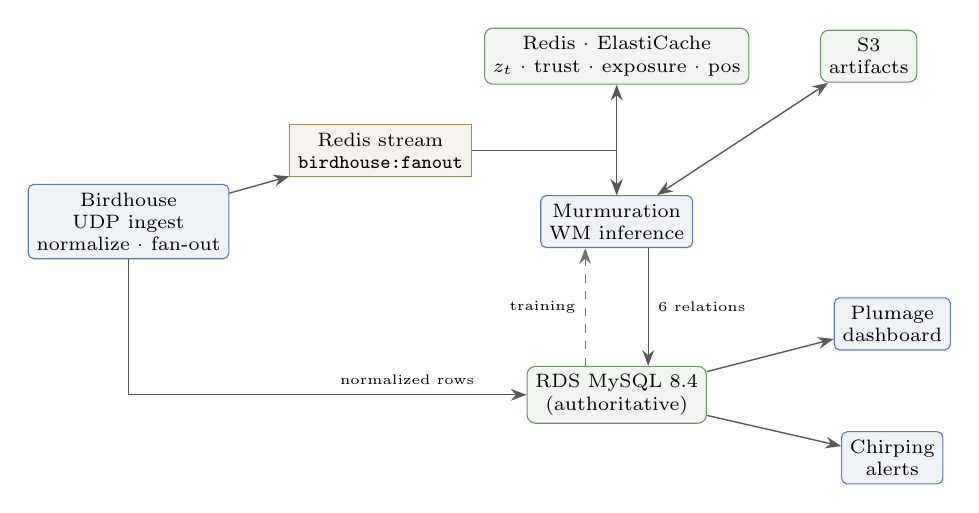
\begin{tikzpicture}[
 store/.style={rectangle, rounded corners=3pt, draw=cgreen!80, fill=cgreen!8,
 align=center, inner sep=3pt, font=\scriptsize},
 svc/.style={rectangle, rounded corners=2pt, draw=cblue!80, fill=cblue!8,
 align=center, inner sep=3pt, font=\scriptsize},
 q/.style={rectangle, draw=cbrown!80, fill=cbrown!8, align=center,
 inner sep=3pt, font=\scriptsize},
 a/.style={-{Stealth[length=2mm]}, draw=black!65, line width=0.5pt},
 aa/.style={{Stealth[length=2mm]}-{Stealth[length=2mm]}, draw=black!65, line width=0.5pt},
 ad/.style={-{Stealth[length=2mm]}, draw=black!55, line width=0.5pt, dashed},
]
 \node[svc] (BH) at (0,1.7) {Birdhouse\\UDP ingest\\normalize · fan-out};
 \node[q] (Q) at (3.2,2.6) {Redis stream\\\texttt{birdhouse:fanout}};
 \node[svc] (WM) at (6.2,1.7) {Murmuration\\WM inference};
 \node[store] (RS) at (6.2,3.8) {Redis · ElastiCache\\$z_t$ · trust · exposure · pos};
 \node[store] (S3) at (9.4,3.8) {S3\\artifacts};
 \node[store] (PDB) at (6.2,-0.5) {RDS MySQL 8.4\\(authoritative)};
 \node[svc] (DASH) at (9.7,0.4) {Plumage\\dashboard};
 \node[svc] (CH) at (9.7,-1.3) {Chirping\\alerts};

 \draw[a] (BH) -- (Q);
 \draw[a] (Q) -| (WM);
 \draw[a] (BH.south) |- (PDB.west) node[pos=0.85,above,font=\tiny]{normalized rows};
 \draw[aa] (WM) -- (RS);
 \draw[aa] (WM) -- (S3);
 \draw[a] ([xshift=4mm]WM.south) -- node[midway,right,font=\tiny]{6 relations} ([xshift=4mm]PDB.north);
 \draw[ad] ([xshift=-4mm]PDB.north) -- node[midway,left,font=\tiny]{training} ([xshift=-4mm]WM.south);
 \draw[a] (PDB) -- (DASH);
 \draw[a] (PDB) -- (CH);
\end{tikzpicture}%
}
\caption{Data flow around Murmuration. Birdhouse writes canonical rows to the
database and fans them out through a Redis stream; the model consumes the fan-out
(off the hot path),
holds fast state $z_t$ and slow per-device state in Redis, loads versioned weights
from S3, and upserts six result relations back to the database, where the
dashboard and Chirping consume them. The dashed edge is the offline training read. Weather
(Thermal) is omitted for clarity; see Table~\ref{tab:io}.}
\label{fig:dataflow}
\end{figure}

\section{Experiments}
\label{sec:exp}
We report twelve studies, in four groups.
\emph{Establishing the bar}: baseline forecasting on a synthetic field, and the
calibration of that baseline's uncertainty (\S\ref{sec:exp}).
\emph{Inputs and instruments}: live static-context extraction, fault injection
against the trust controller, and hierarchical reliability across the device
fleet.
\emph{Clearing the bar}: training the recurrent core, transferring it to real
CAMS PM\textsubscript{2.5}, adding a stochastic latent, rolling it out
autoregressively, and comparing it against a derived ensemble Kalman filter.
\emph{Deployment questions}: how late-arriving data verifies the model for free,
how output credibility depends on fleet size and history, and what several
channels per device buy.
Together they establish the design's inputs, its bar, and a first trained core
that clears it; training on Canarin's own operational data remains future work.

\subsection{Baseline forecasting}
\paragraph{Data.}
We use a synthetic field with genuine spatiotemporal structure: a diurnal base
with two rush-hour peaks, a source plume advected by a slowly rotating wind, a
spatial gradient, and AR(1) sensor noise, over $12$ sensors and $40$ days at
hourly cadence. We average over $30$ independent realizations (seeds) and hold out
the final $25\%$ of each series for testing.

\paragraph{Methods and metric.}
We compare \emph{persistence} ($\hat y_{t+h}=y_t$), \emph{diurnal-persistence}
(persistence plus a train-only hour-of-day climatology correction), and a
\emph{graph-lite} spatiotemporal model: a ridge readout over a device's own recent
anomalies and an inverse-distance neighbour-anomaly message, predicting the
target-time climatology plus a learned correction. The graph-lite model is given
the \emph{same} diurnal information as diurnal-persistence, so the comparison
isolates what spatial and temporal structure adds. Skill is
$1-\mathrm{RMSE}_{\text{model}}/\mathrm{RMSE}_{\text{persistence}}$. For the
virtual-sensor task we hold out each sensor in turn and reconstruct it by
inverse-distance weighting of the others.

\paragraph{Results.}
Table~\ref{tab:forecast} and Fig.~\ref{fig:results} report the results. Both
structured baselines beat persistence by a wide and growing margin as the horizon
lengthens---persistence collapses precisely because it ignores the diurnal
cycle---reaching $53.9\pm4.5\%$ skill for graph-lite at $h=6$. The graph-lite
model overtakes pure diurnal-persistence only at longer horizons, where spatial
propagation of the advected plume carries information the single-site climatology
cannot. The leave-one-out virtual-sensor reconstruction attains
$\mathrm{RMSE}=0.880\pm0.117$. \textbf{The operational lesson is that the
recurrent core must be measured against the graph-lite row, not persistence:} a
strong linear spatiotemporal model already captures roughly half the reducible
error, and that is the bar a heavier model must clear to justify itself
(\S\ref{sec:rssm} shows the trained core clears it at every horizon $\geq2$).

\begin{table}[t]
\centering
\small
\begin{tabular}{@{}c cc cc@{}}
\toprule
& \multicolumn{2}{c}{\textbf{RMSE} (norm.\ units)} & \multicolumn{2}{c}{\textbf{Skill vs persistence}} \\
\cmidrule(lr){2-3}\cmidrule(lr){4-5}
$h$ (h) & diurnal-pers. & graph-lite & diurnal-pers. & graph-lite \\
\midrule
1 & $0.272\pm0.004$ & $0.281\pm0.005$ & $+27.4\pm3.8\%$ & $+25.2\pm3.2\%$ \\
2 & $0.350\pm0.007$ & $0.348\pm0.006$ & $+42.1\pm4.5\%$ & $+42.5\pm4.1\%$ \\
3 & $0.409\pm0.011$ & $0.396\pm0.009$ & $+48.5\pm4.6\%$ & $+50.1\pm4.3\%$ \\
6 & $0.515\pm0.018$ & $0.480\pm0.015$ & $+50.5\pm5.0\%$ & $\mathbf{+53.9\pm4.5\%}$ \\
\midrule
\multicolumn{5}{@{}l}{\footnotesize persistence RMSE: $0.376/0.608/0.799/1.048$ at $h=1/2/3/6$.}\\
\bottomrule
\end{tabular}
\caption{Forecast skill on the synthetic field, mean$\pm$std over 30 seeds.
Graph-lite overtakes diurnal-persistence as the horizon grows, where spatial
propagation matters.}
\label{tab:forecast}
\end{table}

\begin{figure}[t]
\centering
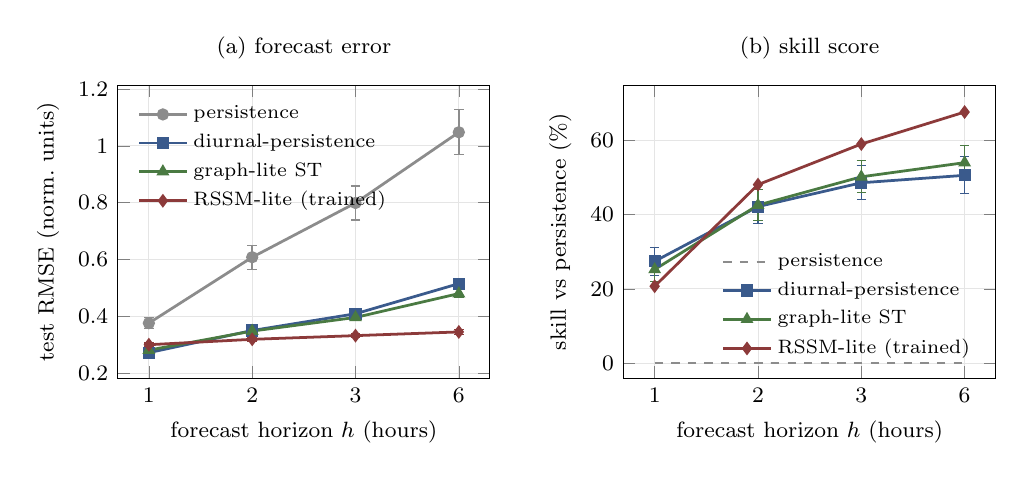
\begin{tikzpicture}
\begin{groupplot}[
 group style={group size=2 by 1, horizontal sep=1.7cm},
 width=0.52\linewidth, height=5.3cm,
 xtick={1,2,3,4}, xticklabels={1,2,3,6}, xmin=0.7, xmax=4.3,
 xlabel={forecast horizon $h$ (hours)},
 tick label style={font=\footnotesize},
 label style={font=\footnotesize},
 title style={font=\footnotesize},
 legend cell align=left,
 legend style={font=\scriptsize, draw=none, fill=none},
 grid=both, grid style={gray!20, line width=0.3pt},
 error bars/error bar style={line width=0.5pt},
 every axis plot/.append style={line width=1pt, mark size=1.7pt},
]
\nextgroupplot[ylabel={test RMSE (norm.\ units)}, title={(a) forecast error},
 legend pos=north west]
\addplot[cgrey, mark=*, mark options={fill=cgrey}, error bars/.cd, y dir=both, y explicit]
 coordinates {(1,0.376)+-(0,0.019) (2,0.608)+-(0,0.042) (3,0.799)+-(0,0.060) (4,1.048)+-(0,0.079)};
\addlegendentry{persistence}
\addplot[cblue, mark=square*, mark options={fill=cblue}, error bars/.cd, y dir=both, y explicit]
 coordinates {(1,0.272)+-(0,0.004) (2,0.350)+-(0,0.007) (3,0.409)+-(0,0.011) (4,0.515)+-(0,0.018)};
\addlegendentry{diurnal-persistence}
\addplot[cgreen, mark=triangle*, mark options={fill=cgreen}, error bars/.cd, y dir=both, y explicit]
 coordinates {(1,0.281)+-(0,0.005) (2,0.348)+-(0,0.006) (3,0.396)+-(0,0.009) (4,0.480)+-(0,0.015)};
\addlegendentry{graph-lite ST}
\addplot[cred, mark=diamond*, mark options={fill=cred}, error bars/.cd, y dir=both, y explicit]
 coordinates {(1,0.300)+-(0,0.006) (2,0.319)+-(0,0.006) (3,0.332)+-(0,0.006) (4,0.345)+-(0,0.009)};
\addlegendentry{RSSM-lite (trained)}

\nextgroupplot[ylabel={skill vs persistence (\%)}, title={(b) skill score},
 legend pos=south east, ymin=-4]
\addplot[cgrey, dashed, line width=0.8pt, mark=none, domain=1:4] {0};
\addlegendentry{persistence}
\addplot[cblue, mark=square*, mark options={fill=cblue}, error bars/.cd, y dir=both, y explicit]
 coordinates {(1,27.4)+-(0,3.8) (2,42.1)+-(0,4.5) (3,48.5)+-(0,4.6) (4,50.5)+-(0,5.0)};
\addlegendentry{diurnal-persistence}
\addplot[cgreen, mark=triangle*, mark options={fill=cgreen}, error bars/.cd, y dir=both, y explicit]
 coordinates {(1,25.2)+-(0,3.2) (2,42.5)+-(0,4.1) (3,50.1)+-(0,4.3) (4,53.9)+-(0,4.5)};
\addlegendentry{graph-lite ST}
\addplot[cred, mark=diamond*, mark options={fill=cred}]
 coordinates {(1,20.7) (2,48.0) (3,58.9) (4,67.5)};
\addlegendentry{RSSM-lite (trained)}
\end{groupplot}
\end{tikzpicture}
\caption{Forecast error (a) and skill over persistence (b) versus horizon, mean
over 30 seeds with $\pm1$ std bars. The persistence baseline (dashed, right) is
the zero-skill reference; the gap between it and graph-lite is what the recurrent
core inherits, and the gap \emph{above} graph-lite is what it must earn. The
trained RSSM-lite core (red, 8 seeds) is overlaid: it falls below graph-lite at
every horizon $\geq2$, earning that gap.}
\label{fig:results}
\end{figure}

\paragraph{Calibration.}
The forecaster above is a point predictor, but the world model will emit
uncertainty bands, so we establish the protocol and a baseline here. We equip
graph-lite ($h=3$) with a predictive variance and measure the empirical coverage
of its central intervals against the nominal level (Table~\ref{tab:calib}). A
single train-residual variance (homoscedastic) is \emph{underconfident}---its
$90\%$ interval covers $98\%$---while a heteroscedastic estimate from a
log-variance regression is \emph{overconfident} ($90\%\!\to\!78\%$); neither is
usable as-is (expected calibration error $\approx0.10$--$0.12$). A one-parameter
recalibration---a single scale factor chosen on a validation slice---restores
coverage almost exactly (error $0.013$). This sets a bar: the recurrent core's
assimilation posterior should be calibrated \emph{without} such a post-hoc fudge,
and this is the protocol by which we will check it.

\begin{table}[t]
\centering
\small
\begin{tabular}{@{}cccc@{}}
\toprule
nominal & homoscedastic & heteroscedastic & recalibrated \\
\midrule
0.50 & 0.658 & 0.382 & 0.520 \\
0.80 & 0.926 & 0.655 & 0.818 \\
0.90 & 0.977 & 0.776 & 0.911 \\
0.95 & 0.992 & 0.853 & 0.955 \\
\midrule
ECE & 0.101 & 0.121 & \textbf{0.013} \\
\bottomrule
\end{tabular}
\caption{Empirical coverage of graph-lite's central prediction intervals versus
the nominal level ($h=3$, 20 seeds); ECE is the mean $|\text{empirical}-\text{nominal}|$. Naive bolt-on variances miscalibrate in both directions; a single
validation-chosen scale factor fixes coverage.}
\label{tab:calib}
\end{table}

\subsection{Static-context extraction (live)}
Table~\ref{tab:static} shows features extracted live for three Paris sites of
contrasting morphology. The dense boulevard site yields a high plan-area index,
high aspect ratio, and low sky-view factor---a poorly ventilated street
canyon---while the park-edge site is correctly resolved as open sky. One site's
building query timed out at the provider and fell back to fleet-median imputation,
exercising the degradation path the pipeline is designed to handle.

\begin{table}[t]
\centering
\small
\begin{tabular}{@{}l r r r r r@{}}
\toprule
Site (Paris) & elev.\ (m) & \#bldg & $\lambda_p$ & aspect & SVF \\
\midrule
Dense boulevard & 51 & 157 & 0.38 & 1.48 & 0.56 \\
Park edge (open) & 48 & 0 & 0.00 & 0.00 & 1.00 \\
Riverside\textsuperscript{$\dagger$} & 36 & --- & \multicolumn{3}{c}{\emph{imputed (provider timeout)}} \\
\bottomrule
\end{tabular}
\caption{Live static-context features. $\lambda_p$: plan-area index; SVF:
sky-view-factor proxy. \textsuperscript{$\dagger$}Building query returned a
gateway timeout; values imputed from the fleet median, as designed.}
\label{tab:static}
\end{table}

\subsection{Fault injection and the trust controller}
\label{sec:faults}
To test the controller's central claim---that it down-weights bad devices without
discarding good ones---we inject the four fault modes of \S\ref{sec:model} into the
synthetic field: a \emph{stuck} flatline, a slow additive \emph{drift}, an
\emph{indoor} device decoupled from the field (low exposure), and a
\emph{mislocated} device reporting the field at the wrong coordinates. On a
36-device network, six devices fail at $t=10$\,d and one drift device recovers at
$t=17.5$\,d. The controller calibrates each device's expected disagreement against
its trust-weighted neighbours during a clean warm-up, then runs the asymmetric-EMA
update of Eq.~\eqref{eq:trust} with a flatline hard gate and a trust floor. We
compare field reconstruction on a $16\times16$ grid under three weightings:
uniform, trust-weighted, and an \emph{oracle} that drops the faulty devices
outright.

Figure~\ref{fig:faults} reports the outcome over 30 seeds. Trust of stuck and
drifting devices collapses within hours to a day or two of onset, healthy
devices stay near one (false-positive rate $8.6\%$), and the recovering drift
device climbs back once its fault clears. Trust weighting cuts reconstruction RMSE
from $0.179$ (uniform) to $0.155$, a $13\%$ reduction that recovers most of the way
to the oracle floor of $0.136$. At the density simulated here the \emph{mislocated}
device is also caught---its neighbours are close enough to contradict a
wrong-location reading---but this is the one result that does not survive
sparsification (see below). The remaining hard case is the pure \emph{indoor} fault:
a device sitting at its baseline only disagrees when the field departs from that
baseline, so it is caught slowly by disagreement alone. This is not a failure of
the controller but evidence for the architecture---reliability and exposure are
orthogonal axes, and an indoor device is an \emph{exposure} problem for the
exposure estimator, not a reliability fault for the trust loop.

\paragraph{A sparser, fully reproducible replication.}
Because the mislocation result is density-sensitive, we re-ran the study
independently on a sparser network (16 devices, four faults, 25 seeds) with a
released script. It reproduces the core findings: the flatline hard gate catches
the stuck device in $\sim$15\,h, drift and indoor within two to three days, healthy
devices are barely touched (mean final trust $0.85$, false-positive rate $3.7\%$),
and trust recovers about $89\%$ of the fault-induced reconstruction error (a
fault-free floor of $0.885$, degraded to $1.329$ without trust and restored to
$0.934$ with it). The one divergence is exactly mislocation: with neighbours
further apart, a device reporting a plausible value from $\sim$1.6\,km away is
caught in only $12\%$ of seeds. Mislocation detection therefore scales with network
density; below it, mislocation is a \emph{position} problem for the position state,
not a \emph{reliability} problem for the trust loop---the empirical face of the
identifiability argument in \S\ref{sec:model}.

\begin{figure}[t]
\centering
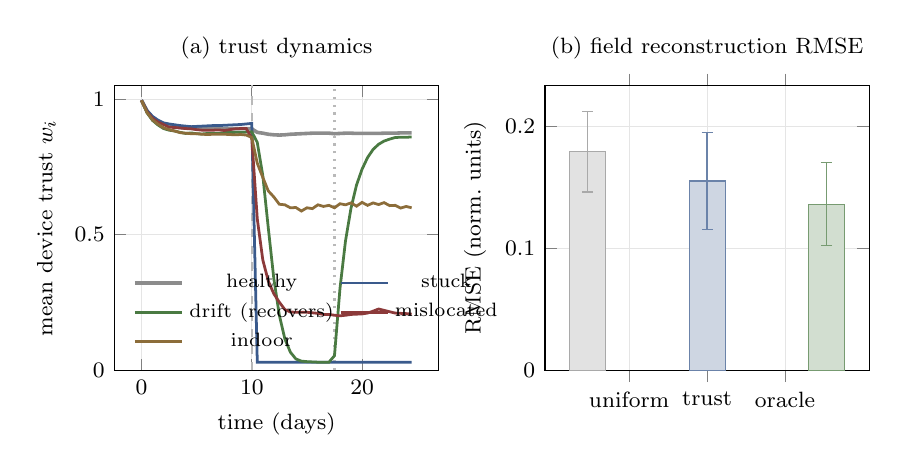
\begin{tikzpicture}
\begin{groupplot}[
 group style={group size=2 by 1, horizontal sep=1.35cm},
 width=0.47\linewidth, height=5.2cm,
 tick label style={font=\footnotesize}, label style={font=\footnotesize},
 title style={font=\footnotesize}, legend style={font=\scriptsize, draw=none, fill=none},
 grid=both, grid style={gray!20, line width=0.3pt},]
\nextgroupplot[xlabel={time (days)}, ylabel={mean device trust $w_i$},
 title={(a) trust dynamics}, ymin=0, ymax=1.05, legend pos=south west, legend columns=2]
\draw[gray!55,dashed,thick] (axis cs:10.00,0) -- (axis cs:10.00,1.05);
\draw[gray!55,dotted,thick] (axis cs:17.50,0) -- (axis cs:17.50,1.05);
\addplot[cgrey, line width=1.3pt] coordinates {(0.00,0.995) (0.50,0.956) (1.00,0.932) (1.50,0.917) (2.00,0.908) (2.50,0.902) (3.00,0.898) (3.50,0.895) (4.00,0.893) (4.50,0.892) (5.00,0.891) (5.50,0.891) (6.00,0.891) (6.50,0.891) (7.00,0.891) (7.50,0.891) (8.00,0.890) (8.50,0.891) (9.00,0.891) (9.50,0.891) (10.00,0.890) (10.50,0.877) (11.00,0.874) (11.50,0.870) (12.00,0.868) (12.50,0.867) (13.00,0.868) (13.50,0.870) (14.00,0.871) (14.50,0.872) (15.00,0.873) (15.50,0.874) (16.00,0.874) (16.50,0.874) (17.00,0.874) (17.50,0.872) (18.00,0.873) (18.50,0.874) (19.00,0.874) (19.50,0.873) (20.00,0.873) (20.50,0.873) (21.00,0.873) (21.50,0.873) (22.00,0.874) (22.50,0.874) (23.00,0.874) (23.50,0.875) (24.00,0.875) (24.50,0.875)};
\addlegendentry{healthy}
\addplot[cblue, line width=1pt] coordinates {(0.00,0.996) (0.50,0.958) (1.00,0.936) (1.50,0.922) (2.00,0.912) (2.50,0.908) (3.00,0.905) (3.50,0.902) (4.00,0.900) (4.50,0.898) (5.00,0.899) (5.50,0.900) (6.00,0.901) (6.50,0.902) (7.00,0.902) (7.50,0.903) (8.00,0.904) (8.50,0.905) (9.00,0.906) (9.50,0.908) (10.00,0.910) (10.50,0.030) (11.00,0.030) (11.50,0.030) (12.00,0.030) (12.50,0.030) (13.00,0.030) (13.50,0.030) (14.00,0.030) (14.50,0.030) (15.00,0.030) (15.50,0.030) (16.00,0.030) (16.50,0.030) (17.00,0.030) (17.50,0.030) (18.00,0.030) (18.50,0.030) (19.00,0.030) (19.50,0.030) (20.00,0.030) (20.50,0.030) (21.00,0.030) (21.50,0.030) (22.00,0.030) (22.50,0.030) (23.00,0.030) (23.50,0.030) (24.00,0.030) (24.50,0.030)};
\addlegendentry{stuck}
\addplot[cgreen, line width=1pt] coordinates {(0.00,0.995) (0.50,0.949) (1.00,0.921) (1.50,0.904) (2.00,0.891) (2.50,0.885) (3.00,0.882) (3.50,0.877) (4.00,0.873) (4.50,0.875) (5.00,0.872) (5.50,0.871) (6.00,0.873) (6.50,0.873) (7.00,0.873) (7.50,0.876) (8.00,0.876) (8.50,0.877) (9.00,0.877) (9.50,0.878) (10.00,0.879) (10.50,0.840) (11.00,0.718) (11.50,0.524) (12.00,0.338) (12.50,0.203) (13.00,0.116) (13.50,0.067) (14.00,0.042) (14.50,0.034) (15.00,0.032) (15.50,0.031) (16.00,0.030) (16.50,0.030) (17.00,0.030) (17.50,0.054) (18.00,0.302) (18.50,0.477) (19.00,0.598) (19.50,0.683) (20.00,0.741) (20.50,0.784) (21.00,0.814) (21.50,0.833) (22.00,0.845) (22.50,0.852) (23.00,0.858) (23.50,0.859) (24.00,0.859) (24.50,0.860)};
\addlegendentry{drift (recovers)}
\addplot[cred, line width=1pt] coordinates {(0.00,0.995) (0.50,0.953) (1.00,0.929) (1.50,0.915) (2.00,0.906) (2.50,0.896) (3.00,0.895) (3.50,0.893) (4.00,0.891) (4.50,0.890) (5.00,0.887) (5.50,0.885) (6.00,0.885) (6.50,0.885) (7.00,0.886) (7.50,0.884) (8.00,0.887) (8.50,0.890) (9.00,0.891) (9.50,0.891) (10.00,0.855) (10.50,0.558) (11.00,0.407) (11.50,0.329) (12.00,0.282) (12.50,0.251) (13.00,0.224) (13.50,0.215) (14.00,0.214) (14.50,0.214) (15.00,0.214) (15.50,0.212) (16.00,0.210) (16.50,0.206) (17.00,0.206) (17.50,0.203) (18.00,0.201) (18.50,0.203) (19.00,0.206) (19.50,0.207) (20.00,0.208) (20.50,0.211) (21.00,0.218) (21.50,0.226) (22.00,0.221) (22.50,0.216) (23.00,0.211) (23.50,0.210) (24.00,0.209) (24.50,0.207)};
\addlegendentry{mislocated}
\addplot[cbrown, line width=1pt] coordinates {(0.00,0.995) (0.50,0.950) (1.00,0.923) (1.50,0.907) (2.00,0.894) (2.50,0.887) (3.00,0.882) (3.50,0.876) (4.00,0.874) (4.50,0.872) (5.00,0.872) (5.50,0.870) (6.00,0.869) (6.50,0.870) (7.00,0.870) (7.50,0.870) (8.00,0.869) (8.50,0.868) (9.00,0.869) (9.50,0.867) (10.00,0.858) (10.50,0.763) (11.00,0.711) (11.50,0.661) (12.00,0.639) (12.50,0.612) (13.00,0.610) (13.50,0.599) (14.00,0.600) (14.50,0.587) (15.00,0.599) (15.50,0.596) (16.00,0.610) (16.50,0.604) (17.00,0.608) (17.50,0.599) (18.00,0.614) (18.50,0.610) (19.00,0.617) (19.50,0.605) (20.00,0.619) (20.50,0.608) (21.00,0.617) (21.50,0.611) (22.00,0.618) (22.50,0.607) (23.00,0.608) (23.50,0.598) (24.00,0.604) (24.50,0.599)};
\addlegendentry{indoor}
\nextgroupplot[title={(b) field reconstruction RMSE}, ylabel={RMSE (norm.\ units)},
 ybar, bar width=13pt, xtick={1,2,3}, xticklabels={uniform,trust,oracle},
 xmin=0.4, xmax=3.6, ymin=0, enlarge x limits=0.15,
 error bars/error bar style={line width=0.6pt}]
\addplot[cgrey!75, fill=cgrey!25, error bars/.cd, y dir=both, y explicit] coordinates {(1,0.179) +- (0,0.033)};
\addplot[cblue!75, fill=cblue!25, error bars/.cd, y dir=both, y explicit] coordinates {(2,0.155) +- (0,0.040)};
\addplot[cgreen!75, fill=cgreen!25, error bars/.cd, y dir=both, y explicit] coordinates {(3,0.136) +- (0,0.034)};
\end{groupplot}
\end{tikzpicture}
\caption{Trust controller under injected faults: 30 seeds, 36 devices, six
faults from $t=10$\,d, with the drift sensor recovering at $t=17.5$\,d (dotted).
(a)~Category-mean trust. Healthy devices stay near one; stuck, drift and
mislocated devices lose trust; the drift sensor recovers once its fault clears.
Pure \emph{indoor} (exposure) faults are slowest to catch by disagreement alone,
motivating the separate exposure estimator. (b)~Field-reconstruction RMSE. Trust
weighting ($0.155$) improves on uniform ($0.179$, $-13\%$) and approaches the
oracle that drops faulty devices outright ($0.136$).}
\label{fig:faults}
\end{figure}

\subsection{Reliability across the device hierarchy}
\label{sec:hier}
Section~\ref{sec:model} argued that reliability should be pooled across the
type\,$\to$\,device-model\,$\to$\,instance hierarchy; we test that on a simulated
fleet of six device models, eight instances each, one of which is a defective
revision (a systematic low-reliability shift). Each instance yields noisy agreement
measurements; half are \emph{mature} (many observations) and half \emph{cold}
(few). We estimate each instance's reliability three ways---no pooling (instance
alone), complete pooling (one fleet value), and partial pooling (two-level
empirical-Bayes shrinkage)---and score against ground truth
(Table~\ref{tab:hier}).

Partial pooling is best overall and decisively so where it matters: on cold
instances it nearly halves the error of estimating each alone ($0.27$ vs $0.57$),
because a data-poor unit borrows strength from its device model. For a brand-new
instance with no observations, its device-model posterior is a far better prior
than the fleet mean (RMSE $0.29$ vs $0.87$)---the cold-start benefit the deployed
system needs. The defective revision is correctly identified as the
lowest-reliability model in $93\%$ of runs, separating \emph{``this revision is
biased''} from \emph{``this unit is broken.''} As expected, for \emph{mature}
instances plain estimation is marginally better ($0.16$ vs $0.19$): once a unit has
enough data of its own, shrinkage adds a little bias, so the pooling correctly
fades as observations accumulate.

\begin{table}[t]
\centering
\small
\begin{tabular}{@{}lccc@{}}
\toprule
& \multicolumn{3}{c}{reliability RMSE (lower is better)} \\
\cmidrule(lr){2-4}
estimator & all & cold ($n{=}3$) & mature ($n{=}40$) \\
\midrule
no pooling & 0.418 & 0.570 & \textbf{0.156} \\
complete pooling & 0.872 & 0.869 & 0.874 \\
partial pooling (EB) & \textbf{0.235} & \textbf{0.269} & 0.187 \\
\bottomrule
\end{tabular}
\caption{Per-instance reliability estimation on a simulated fleet (300 seeds).
Partial pooling across the device hierarchy wins overall and on data-poor cold
instances; for data-rich mature instances estimating each alone is marginally
better, as hierarchical shrinkage predicts.}
\label{tab:hier}
\end{table}

\subsection{Training the recurrent core}
\label{sec:rssm}
The baselines set a bar; here we clear it. We implement the dynamics core $M$ as a
deterministic-latent gated recurrent unit (an RSSM-lite core, without the stochastic
latent) that encodes the whole sensor field's history into a latent $h_t$ and
decodes it with a direct readout head per horizon. It is trained on the synthetic
field by back-propagation through time---hand-derived and gradient-checked to
$3\times10^{-9}$, as no autodiff framework was available---seeing only observations
and hour-of-day, the \emph{same} information as graph-lite, with the hidden wind
forcing withheld to keep the comparison fair. Table~\ref{tab:rssm} and
Fig.~\ref{fig:results} report the result over 8 seeds.

The recurrent core clears the graph-lite bar at every horizon beyond one step, and
the margin widens with lead time: at $h=6$ it cuts RMSE from $0.475$ to $0.345$, a
$27\%$ relative reduction, for $+67.5\%$ skill over persistence against graph-lite's
$+55.2\%$. The mechanism is the one the design predicts---a recurrent latent
captures the advective dynamics, so its forecasts degrade far more slowly than a
memoryless linear readout. At $h=1$ the cheap baseline stays marginally sharper
($0.280$ vs $0.300$): a one-step nowcast has little dynamics to model, and the
linear anomaly-plus-climatology readout is hard to beat there. This is the paper's
central premise with evidence on synthetic data: the recurrent core earns its place
precisely where multi-step field evolution matters.

\begin{table}[t]
\centering
\small
\begin{tabular}{@{}c ccc c@{}}
\toprule
& \multicolumn{3}{c}{\textbf{test RMSE} (norm.\ units)} & \\
\cmidrule(lr){2-4}
$h$ (h) & persistence & graph-lite & RSSM-lite & $\Delta$ skill \\
\midrule
1 & 0.378 & \textbf{0.280} & $0.300\pm0.006$ & $-5.4$ pp \\
2 & 0.614 & 0.346 & $\mathbf{0.319\pm0.006}$ & $+4.3$ pp \\
3 & 0.809 & 0.394 & $\mathbf{0.332\pm0.006}$ & $+7.6$ pp \\
6 & 1.059 & 0.475 & $\mathbf{0.345\pm0.009}$ & $+12.3$ pp \\
\bottomrule
\end{tabular}
\caption{Trained RSSM-lite core versus baselines (8 seeds). $\Delta$ skill is the
recurrent core's skill-vs-persistence minus graph-lite's, in percentage points. The
core beats graph-lite at every horizon $\geq2$ by a widening margin; at $h=1$ the
linear baseline is marginally better.}
\label{tab:rssm}
\end{table}

\subsection{Beyond the synthetic field: real PM\textsubscript{2.5}}
\label{sec:real}
A trained core that beats a baseline on the very field it was tuned against proves
little unless the advantage transfers. We therefore repeat the forecasting
comparison on data we did not design: hourly PM\textsubscript{2.5} from the CAMS
European air-quality analysis (via a public API) at 16 locations across greater
Paris over 90 days. This is a modeled, gap-free, fault-free product---smooth and
highly spatially correlated (mean inter-location correlation $0.94$)---so it
exercises the forecasting core, not the fault or reliability machinery, and it is
not Canarin's own Plumage stream, which we cannot access from here. The harness,
split, and core are otherwise unchanged; the core is averaged over four
initializations.

The mid-horizon advantage transfers (Table~\ref{tab:real}). The recurrent core
clearly beats graph-lite at $h=2$ and $h=3$ ($0.76$ vs $0.83$ and $0.98$ vs $1.06$
$\mu$g/m$^3$) and edges it at $h=6$; at $h=1$, real PM\textsubscript{2.5} is so
autocorrelated that plain persistence wins and every model sits within a few percent
of it. The margins are smaller than on the synthetic field---unsurprisingly, as the
CAMS product is spatially smooth, offering less advective structure for a recurrent
latent to exploit than the synthetic plume---but the ordering that matters holds on
real data: the recurrent core earns its place at the horizons where field evolution,
not mere persistence, drives the forecast.

\begin{table}[t]
\centering
\small
\begin{tabular}{@{}c cccc cc@{}}
\toprule
& \multicolumn{4}{c}{\textbf{test RMSE} ($\mu$g/m$^3$)} & \multicolumn{2}{c}{skill vs pers.} \\
\cmidrule(lr){2-5}\cmidrule(lr){6-7}
$h$ & persist. & diurnal & graph-lite & RSSM-lite & RSSM & g-lite \\
\midrule
1 & 0.54 & \textbf{0.50} & 0.55 & 0.55 & $-2.4\%$ & $-2.1\%$ \\
2 & 0.90 & 0.83 & 0.83 & \textbf{0.76} & $+15.4\%$ & $+8.0\%$ \\
3 & 1.20 & 1.09 & 1.06 & \textbf{0.98} & $+17.9\%$ & $+11.5\%$ \\
6 & 1.78 & 1.62 & 1.50 & \textbf{1.48} & $+16.8\%$ & $+15.8\%$ \\
\bottomrule
\end{tabular}
\caption{Forecasting on real CAMS PM\textsubscript{2.5} (16 locations across greater
Paris, 90 days; RSSM over 4 inits). The recurrent core's mid-horizon advantage over
graph-lite transfers to real data; at $h=1$ persistence dominates highly
autocorrelated PM\textsubscript{2.5}.}
\label{tab:real}
\end{table}

\subsection{A probabilistic core and its calibration}
\label{sec:calibcore}
The design promises calibrated uncertainty from the core's posterior; we test that
directly. We give the recurrent core a stochastic latent---a reparameterized
Gaussian $z_t\sim\mathcal{N}(\mu(h_t),\sigma(h_t)^2)$ regularized toward
$\mathcal{N}(0,I)$---and a heteroscedastic Gaussian decoder that outputs a mean
\emph{and} a variance per horizon, trained by an ELBO (negative log-likelihood
$+\,\beta\,$KL; hand-derived gradients, checked to $4\times10^{-9}$). Predictive
bands come from Monte-Carlo over the latent via the law of total variance. Point
accuracy is unchanged from the deterministic core (RMSE $0.30/0.33/0.34/0.35$ at
$h=1/2/3/6$), so probabilistic training costs nothing in sharpness.

Two honest findings follow (Table~\ref{tab:calibcore}). First, on this mostly
\emph{observed} forecasting task the latent \emph{collapses}: it supplies under
$1\%$ of the predictive variance. With direct per-horizon heads the heteroscedastic
decoder already captures horizon-dependent spread, so the latent is redundant;
realizing uncertainty that grows with horizon requires rolling the state forward
autoregressively rather than reading each lead off a static head, which we do next
(\S\ref{sec:rollout}). Second, the
decoder's \emph{raw} bands are overconfident---a $90\%$ interval covers $77\%$ (ECE
$0.13$)---because a variance fit to training residuals under-covers the larger
errors on held-out data, the same scale gap the naive baselines showed in
\S\ref{sec:exp}. A single per-horizon recalibration on a validation slice fixes it
(ECE $0.13\!\to\!0.03$; the $90\%$ interval $0.77\!\to\!0.92$). This corrects an
over-optimistic reading of the design: the trained core does not emit calibrated
bands ``for free''; it emits well-\emph{shaped}, input- and horizon-dependent bands
whose \emph{scale} still needs a one-parameter recalibration.

\begin{table}[t]
\centering
\small
\begin{tabular}{@{}ccc@{}}
\toprule
nominal & raw bands & recalibrated \\
\midrule
0.50 & 0.379 & 0.537 \\
0.80 & 0.648 & 0.829 \\
0.90 & 0.766 & 0.915 \\
0.95 & 0.841 & 0.957 \\
\midrule
ECE & 0.129 & \textbf{0.030} \\
\bottomrule
\end{tabular}
\caption{Calibration of the probabilistic core's predictive intervals (synthetic
field, 4 seeds, coverage averaged over horizons). The trained core's raw bands are
overconfident; a one-parameter per-horizon recalibration on a validation slice
restores coverage, matching the protocol of \S\ref{sec:exp}.}
\label{tab:calibcore}
\end{table}

\subsection{Autoregressive rollout: uncertainty that compounds}
\label{sec:rollout}
The direct-head core reads every horizon off one latent, so its bands cannot grow
with lead time on their own and its latent sat idle. We therefore replace the four
static heads with a single \emph{one-step} heteroscedastic model---$o_{t+1}\sim
\mathcal{N}(m(h_t),\exp lv(h_t))$, trained by one-step NLL (gradients checked to
$2\times10^{-7}$)---and forecast by \emph{rolling it forward}: sample $o_{t+1}$,
feed it back with the known next-hour features, advance the GRU, sample $o_{t+2}$,
and so on. With $S=60$ sampled trajectories per start, the ensemble spread at $t+k$
is the predictive band.

Now the bands \emph{compound} (Table~\ref{tab:rollout}): the mean predictive
standard deviation grows monotonically with horizon ($0.245\!\to\!0.321$ in
standardized units), because each step's noise is carried forward through the
recurrence---exactly the behaviour a static head cannot produce. Two things follow.
The raw bands are still overconfident (a one-step variance fit to training residuals
under-covers), but \emph{uniformly} so across horizons---raw $90\%$ coverage is
$0.71$--$0.74$ at every lead---so a \emph{single global} scale recalibrates all
horizons at once, reaching ECE $0.013$, better than the direct head's $0.030$ which
needed a separate scale per horizon. The cost is honest: rolling out compounds
error, so point accuracy slips relative to the direct head ($h=6$ RMSE $0.38$ vs
$0.35$) while still beating graph-lite ($0.47$). The rollout thus fixes the
\emph{shape} of the uncertainty; the remaining global offset is removed by a single
validation-chosen scale, and---as we show next---that scale suffices even
conditionally.

\paragraph{The global scale is enough, conditionally too.}
One might worry that a single scale merely trades over-coverage in calm periods
against under-coverage in volatile ones. It does not. Splitting the test starts by
local volatility (the mean absolute one-step change at the forecast origin), the
recalibrated $90\%$ bands cover $0.908$, $0.905$, and $0.906$ in the calm, medium,
and volatile terciles---flat to within $0.001$---and a per-regime scale does not
improve on this. The offset the global scale removes is therefore a benign
\emph{constant}, not a conditional failure. A learned latent-space process-noise
term (the full RSSM) would still matter for predictive distributions that are
non-Gaussian or multi-modal---which the observation-space Gaussian rollout cannot
represent---but for the \emph{coverage} of these bands it is not required.

\begin{table}[t]
\centering
\small
\begin{tabular}{@{}c cc cc@{}}
\toprule
& \multicolumn{2}{c}{predictive band} & \multicolumn{2}{c}{point RMSE} \\
\cmidrule(lr){2-3}\cmidrule(lr){4-5}
$h$ & band std & raw 90\% cov. & rollout & graph-lite \\
\midrule
1 & 0.245 & 0.744 & 0.290 & \textbf{0.280} \\
2 & 0.269 & 0.711 & \textbf{0.343} & 0.346 \\
3 & 0.284 & 0.708 & \textbf{0.369} & 0.393 \\
6 & 0.321 & 0.742 & \textbf{0.384} & 0.473 \\
\bottomrule
\end{tabular}
\caption{Autoregressive rollout (synthetic field, 4 seeds, $S=60$). The predictive
band grows with horizon---uncertainty compounds through the recurrence---and raw
$90\%$ coverage is roughly uniform across horizons, so one global scale recalibrates
all leads (ECE $0.166\!\to\!0.013$). Rolling out slightly worsens point accuracy
versus the direct-head core but still beats graph-lite at $h\geq2$.}
\label{tab:rollout}
\end{table}

\subsection{Derived versus learned: an ensemble Kalman filter on the same field}
\label{sec:enkf}
The paper claims the world model is Bayesian filtering with a learned update rule
(\S\ref{sec:model}). We make the claim testable by running a genuine ensemble
Kalman filter on the same synthetic field, with the same information: a
linear-Gaussian model whose AR coefficient and noise variances are fitted on the
training split, an $80$-member ensemble, covariance inflation, and perturbed-observation
updates. Where the learned core discovers its gate values, the EnKF derives its
gain $K=P(P+R)^{-1}$ from covariances.

One implementation detail is worth recording because it decides whether the
comparison means anything. Fitting a free $12\times12$ process covariance from the
training residuals yields a nearly diagonal matrix (mean off-diagonal correlation
$0.06$), so the gain is diagonal, every sensor is filtered in isolation, and an
observation informs nobody but itself---a faulty device then cannot contaminate its
neighbours, and all fault scenarios return identical numbers. Operational
assimilation avoids this by \emph{modelling} the covariance with a spatial
correlation function rather than fitting it; substituting a Gaussian kernel with a
$1.5$\,km length scale raises the mean off-diagonal correlation to $0.32$ and
restores the spatial information flow that makes assimilation assimilation.

\paragraph{The trade is accuracy against calibration.}
Table~\ref{tab:enkf} gives the comparison. The EnKF matches the linear graph-lite
baseline almost exactly at every horizon---unsurprising, since both are linear
models of the same field---and it is marginally the better nowcaster, beating the
learned core by $5\%$ at $h=1$. But it falls behind badly as the horizon grows: at
$h=6$ the learned core is $28\%$ better ($0.345$ against $0.477$), because a
fitted AR-plus-diffusion transition cannot represent advection the way a learned
recurrence can.

The calibration comparison runs the other way, and this is the honest cost of
learning. The EnKF's $90\%$ intervals cover $0.896$--$0.934$ against a nominal
$0.90$, a mean calibration error of $0.022$, \emph{with no tuning at all}: a
correct Bayesian posterior is calibrated by construction. The learned rollout's raw
bands cover only $0.71$--$0.74$ (error $0.174$) and require the one-parameter
rescaling of \S\ref{sec:rollout} to reach $0.013$. Learning buys a large gain in
multi-step accuracy and gives up calibration-by-construction in exchange.

\paragraph{Two attempts to close the gap in the filter's favour.}
A linear filter beaten by a learned one may simply have been under-specified, so
we tried twice to give the EnKF the physics. Neither attempt helped, and both are
informative. First we replaced the AR transition with an \emph{advection operator}
driven by the known wind, each site inheriting the anomaly from its upwind
footprint. The fitted advection speed came out at \emph{zero}: the synthetic
plume rotates about a fixed source rather than translating, so a spatial-shift
operator has nothing to act on, and the variant reduced to the AR case with an
extra fitted parameter ($0.499$ against $0.477$ at $h=6$). Second we gave the
filter the wind directly, conditioning the climatology on wind sector as well as
hour-of-day---information the recurrent core was denied and had to infer. This was
\emph{worse} at every horizon ($0.374$ against $0.286$ at $h=1$), because
$24\times8$ conditional buckets overfit the available history. The recurrent core's
advantage therefore does not come from being told more, but from learning a
smooth, parameter-efficient representation of a slowly varying hidden regime where
a non-parametric conditional mean cannot. We report the $28\%$ margin as earned.

\paragraph{Adaptive noise estimation is not free.}
The classical counterpart of our trust controller is an adaptive filter that
re-estimates each sensor's observation variance from its own innovations. We
implemented it, and it \emph{degraded} performance in every scenario---including
the faulted ones it was meant to help ($0.326$ against $0.290$ at $h=1$ under a
stuck sensor)---because the variance estimates are noisy at a 48-hour window and
inflate $R$ for healthy sensors along with faulty ones. This is evidence for the
stabilizers of \S\ref{sec:model} rather than against adaptation: the trust
controller is not merely adaptive $R$, but adaptive $R$ with an asymmetric rate, a
floor, a hard gate for unambiguous faults, and periodic forced-listening probes.
Without that machinery, adapting the observation noise costs more than it returns.

\begin{table}[t]
\centering
\small
\begin{tabular}{@{}c cccc cc@{}}
\toprule
& \multicolumn{4}{c}{test RMSE (norm.\ units)} & \multicolumn{2}{c}{$90\%$ coverage} \\
\cmidrule(lr){2-5}\cmidrule(lr){6-7}
$h$ & EnKF & graph-lite & learned core & rollout & EnKF & rollout (raw) \\
\midrule
1 & 0.286 & \textbf{0.281} & 0.300 & 0.290 & 0.896 & 0.744 \\
2 & 0.344 & 0.348 & \textbf{0.319} & 0.343 & 0.920 & 0.711 \\
3 & 0.389 & 0.396 & \textbf{0.332} & 0.369 & 0.928 & 0.708 \\
6 & 0.477 & 0.480 & \textbf{0.345} & 0.384 & 0.934 & 0.742 \\
\midrule
\multicolumn{5}{@{}l}{calibration error at $90\%$} & \textbf{0.022} & 0.174 \\
\bottomrule
\end{tabular}
\caption{A derived filter against a learned one on the same field. The EnKF tracks
the linear baseline and is the better nowcaster, but the learned core is $28\%$
better at six hours. The EnKF is calibrated with no tuning; the learned model's raw
bands are not, and need the rescaling of \S\ref{sec:rollout} (which reaches
$0.013$). This is the trade the architecture makes.}
\label{tab:enkf}
\end{table}

\subsection{Late data as free verification}
\label{sec:lateverif}
The event-time rule of \S\ref{sec:modeldb} forbids late-arriving records from
moving live state or trust. That constraint returns something valuable. While a
device was unreachable, every estimate at its location was formed \emph{without}
its readings; when the buffer flushes, we hold a prediction and an observation
that never informed it. This is an uncontaminated out-of-sample pair at a real
location with real ground truth---precisely the virtual-sensor claim, which is
otherwise the hardest thing in the system to verify, because unmonitored points
have no truth by definition. Outages manufacture it, and an open network with
intermittent connectivity manufactures a great deal of it.

Simulating outages on the real Paris series and scoring the trust-weighted
inverse-distance estimate at each silent device gives an RMSE of
$0.60$\,$\mu$g/m$^3$ with a bias of $-0.03$, and predictive intervals that are
close to nominal on operationally held-out data ($0.90\!\to\!0.94$). That is a
verification of the virtual-sensor product against truth it never saw, obtained
without holding anything back on purpose.

\paragraph{Trust must weight the target, not only the inputs.}
A late reading is evidence only if the device was sound. Scoring against devices
carrying an injected gain or drift fault reports an RMSE of $4.30$ and a $90\%$
coverage of $0.011$; the \emph{same} predictions scored against the true field
give $0.59$. The model appears seven times worse than it is because the yardstick
is broken. Since the gate forbids learning trust from late data, the weight must
come from trust as it stood when the device fell silent, together with the
device-local physical gates of \S\ref{sec:multi}, which need no model and apply
perfectly well to a stale record.

\paragraph{The sample is not random, and the bias is spatial.}
Data is usually late because of connectivity, and connectivity is a property of
the \emph{site}: signal quality in a basement, behind thick walls, or at the
sparse edge of the network is chronically poor rather than occasionally so. The
resulting bias is therefore spatial and persistent rather than temporal and
transient. Restricting verification to the least-connected sites raises RMSE from
$0.52$ to $0.67$ and drops $90\%$ coverage from $0.935$ to $0.890$---about a
$29\%$ pessimistic skew. The direction is fortunate, since late-data verification
understates the model rather than flattering it, and the spatial form is the more
tractable one: a chronic per-site property can be measured and stratified, where a
weather-driven bias could only be guessed at. Scores should be reported per site
group alongside the fleet figure.

\paragraph{Chronic lateness is a coverage gap, not only a verification bias.}
A device that habitually flushes hours after the fact never contributes to the
live cycle. Its own location is therefore served as a virtual estimate
\emph{despite being physically instrumented}, and at the densities an early
deployment actually reaches, nothing recovers it: in our 16-device Paris fleet no
site has a neighbour within 2\,km, so removing a device's own reading leaves its
location supported by little more than the regional mean. This exposed an error in
the credibility score of \S\ref{sec:credibility}, which counted devices by
enrolment. Fleet size must be counted by \emph{timeliness}---the sum of per-device
on-time fractions rather than a headcount---or a fleet whose least-connected
members rarely arrive in time will advertise support it does not provide. On a
plausible connectivity profile, sixteen enrolled devices amount to an effective
fleet of $11.7$.

\subsection{How much should a Plumage user trust an output?}
\label{sec:credibility}
Every relation Murmuration writes is rendered in Plumage beside real
measurements, where a forecast from a four-device, one-week deployment looks
exactly like one from a mature fleet. Since Canarin's fleet is open and grows
over time, the evidence behind an output varies continuously, and the platform
should say so. We therefore measure how output quality actually depends on the
two observable properties of a deployment---\emph{fleet size} $N$ and
\emph{history length} $D$---and derive a credibility score from the measured
curves rather than asserting a formula.

Two findings shape the score (Table~\ref{tab:cred}). First, the two output
families degrade for \emph{different} reasons. Off-device
\emph{virtual-sensor} estimates are fleet-limited: leave-one-out reconstruction
error falls from $1.03$ at $N=4$ to $0.74$ at $N=24$ and is almost insensitive to
history. Forecasts \emph{at} device locations behave oppositely---the linear
baseline's skill is nearly flat in both $N$ and $D$. Second, and decisively for
deployment, the \emph{trained core} is history-hungry in a way the baseline is
not: with 12 devices its $h{=}3$ RMSE is $0.496$ at one week---\emph{worse} than
graph-lite's $0.422$---then $0.376$ at two weeks, $0.336$ at one month and
$0.317$ at three. There is thus a crossover near two weeks below which the
heavier model does not deserve to be served at all.

This yields an operational rule rather than a decoration. Each written row
carries a \texttt{credibility} score in $[0,1]$ and a band; the score weights
history over fleet for forecasts and per-device state ($0.7/0.3$) and fleet plus
\emph{local} density over history for virtual sensors ($0.7/0.3$, scaled by the
number of devices within $\sim$1\,km, so an extrapolated point is never presented
as an interpolated one); and it is multiplied by the mean trust and coverage of
the contributing devices, which the platform already tracks. Two hard floors
apply: under 14 days of history, or under four devices, the score is capped at
$0.20$ and the accompanying note instructs the caller to serve the linear
baseline and label the output provisional. A deployment of 12 devices with 90
days scores $0.96$ for forecasts but only $0.71$ for virtual sensors---the honest
asymmetry a single global confidence number would hide.

\begin{table}[t]
\centering
\small
\begin{tabular}{@{}l ccccc@{}}
\multicolumn{6}{@{}l}{\emph{(a) what limits each output family}}\\
\toprule
& \multicolumn{5}{c}{history $D$ (days), at $N=12$} \\
\cmidrule(lr){2-6}
$h{=}3$ RMSE & 7 & 14 & 30 & 90 & \\
\midrule
graph-lite & 0.422 & 0.399 & 0.402 & 0.397 & \\
trained core & 0.496 & \textbf{0.376} & \textbf{0.336} & \textbf{0.317} & \\
\midrule
& \multicolumn{5}{c}{fleet size $N$} \\
\cmidrule(lr){2-6}
virtual-sensor RMSE & \multicolumn{1}{c}{4} & \multicolumn{1}{c}{6}
 & \multicolumn{1}{c}{8} & \multicolumn{1}{c}{16} & \multicolumn{1}{c}{24} \\
\midrule
(leave-one-out) & 1.034 & 0.913 & 0.807 & 0.796 & 0.760 \\
\bottomrule
\end{tabular}\\[5pt]
\begin{tabular}{@{}ccccl@{}}
\multicolumn{5}{@{}l}{\emph{(b) resulting credibility score}}\\
\toprule
fleet & days & forecast & virtual sensor & band / action \\
\midrule
4 & 7 & 0.10 & 0.18 & low --- serve baseline, mark provisional \\
6 & 14 & 0.38 & 0.37 & medium \\
12 & 30 & 0.73 & 0.63 & high \\
12 & 90 & 0.96 & 0.71 & high \\
24 & 90 & 1.00 & 0.78 & high \\
\bottomrule
\end{tabular}
\caption{Credibility of model outputs. (a)~The trained core needs roughly two
weeks of history before it beats the linear baseline, while virtual sensors are
limited by fleet size and barely improve with history. (b)~The derived score,
which the platform writes alongside every row; forecasts and virtual sensors are
scored separately because they are limited by different things.}
\label{tab:cred}
\end{table}

\subsection{Multiple channels per device}
\label{sec:multi}
Canarin devices report many channels at once (Table~\ref{tab:channels}), so we test
what joint modelling buys \emph{using only channels a Pico actually reports}: the
Plantower's PM\textsubscript{2.5} and PM\textsubscript{10}, and the BME sensors'
humidity and pressure. We take them over the same 16 greater-Paris locations and
90-day window as \S\ref{sec:real}---particulate from the CAMS analysis, humidity and
pressure from the meteorological analysis, joined on timestamp exactly as the
weather block is joined in deployment. PM\textsubscript{1}, the VOC index and the
raw gas signals have no gridded reference product and are not evaluated here.

\paragraph{Correlation is the wrong criterion; predictive gain is the right one.}
Something must decide which channels belong together. Correlation is actively
misleading. We measure instead the \emph{predictive gain}: the percentage RMSE
reduction in forecasting channel $a$ at $h=6$ when a few lags of channel $b$
\emph{from the same device} are added to $a$'s own lags---ridge regressions only,
no core training. The verdicts nearly invert (Table~\ref{tab:multi}a).
PM\textsubscript{2.5} and PM\textsubscript{10} correlate at $0.90$ yet the gain is
$-0.9\%$: each already predicts itself and the other adds nothing. Humidity
correlates with PM\textsubscript{2.5} at just $0.09$ yet yields the largest gain in
the matrix, $+4.9\%$---the hygroscopic-growth coupling that makes an optical
particulate count depend on ambient moisture. Correlation measures co-movement;
what a grouping needs is \emph{incremental information}.

\paragraph{Information is not capacity: covariates must condition, not join.}
The natural next step---put the informative channel into the model---fails, and how
it fails is instructive (Table~\ref{tab:multi}b). Adding humidity as an extra
\emph{target} costs $13\%$ on PM\textsubscript{2.5}; adding it as a global
\emph{input} only, with heads still restricted to the particulate channels, costs
$18\%$; adding pressure too costs $42\%$; one shared core over all four costs
$26\%$. Yet the ridge says the information is real. The discrepancy is dimensional:
the ridge used three lags of \emph{one device's own} humidity, whereas the flat core
appends one input per device per channel, adding parameters that must be learned
from the same limited history. The information is local and per-device; a global
vector state cannot express it. This is direct empirical support for the
architecture of \S\ref{sec:model}---covariates belong in the per-device conditioning
path of the graph encoder, gating how device $i$'s own reading is assimilated,
rather than in the shared latent---and a limitation of the flat RSSM-lite
instantiation used throughout these experiments, which has no per-device structure
to condition.

\paragraph{The right way in is multiplicative, not additive.}
The failure above is not that the information is unusable but that concatenation
is the wrong channel for it. Hygroscopic growth is \emph{multiplicative}: an
optical counter over-reports by a factor that depends on humidity. Applying the
standard growth form as a correction to the observation,
$\text{PM}_{\text{dry}}=\text{PM}_{\text{wet}}/(1+\kappa\,\text{RH}/(1-\text{RH}))$
with a single fitted $\kappa=0.05$, recovers $+4.5\%$---almost exactly the $+4.9\%$
the ridge said was available---at the cost of \emph{one parameter} rather than one
input dimension per device, and it neutralizes the dependence it was meant to
remove (correlation between particulate mass and humidity moves from $+0.079$ to
$-0.043$). This is the design's own claim demonstrated: a covariate belongs in the
observation model, correcting the reading, not in the shared latent as another
predictor. On real optical hardware the effect should be larger than measured
here, since the CAMS product is a model rather than a humidity-sensitive
instrument.

\paragraph{How a hard gate crosses a tranche boundary.}
Two kinds of cross-channel relation must not be conflated. \emph{Statistical}
coupling decides tranche membership and is soft, continuous and measured by
predictive gain. A \emph{physical} constraint such as
$\text{PM}_{1}\!\le\!\text{PM}_{2.5}\!\le\!\text{PM}_{10}$ is hard, conclusive and
indifferent to the partition---and indeed our own assignment places
PM\textsubscript{2.5} and PM\textsubscript{10} in \emph{separate} tranches, so the
constraint spans a boundary the partition just created.

That is not a conflict, because gates do not act in the tranche layer at all. They
run on the raw record, per device and per timestamp, before any tranche sees the
data; needing no model, no neighbour and no history is precisely their value. What
a gate cannot do is \emph{attribute}: a violated inequality proves one of the two
channels is wrong without saying which, and inflating the fine fraction produces
exactly the same violation as deflating the coarse one.

Attribution is where the tranches earn their place. Each channel is scored by the
standardized residual against its own expectation, and the channel that broke its
own pattern is the culprit; the verdict then reaches every tranche through the
shared per-(device,\,channel) trust weight rather than through any latent state.
One detail decides whether this works. An expectation that uses the device's
\emph{own} history absorbs a persistent fault within a step or two, the residual
collapses, and attribution falls to chance---measured at $52\%$ for a sustained
low-reading fault. Built from neighbours only, the expectation cannot adapt to the
device's own fault, and attribution is exact ($100\%$ on both a fine-fraction gain
fault and a coarse-fraction low fault, with the gate itself firing on $72$--$86\%$
of faulted steps and never once in $34{,}560$ clean device-hours). A cross-check
must not be self-referential.

\paragraph{Consequences for tranches.}
Two rules follow, both implemented in the released code. Tranches partition
\emph{targets} only: humidity and pressure are covariates and never become tranche
members. And within the targets, membership follows measured gain, which on this
data leaves PM\textsubscript{2.5} and PM\textsubscript{10} in \emph{separate}
tranches despite their $0.90$ correlation---the opposite of what correlation-based
grouping would do, and consistent with a shared core over the two degrading both.

\begin{table}[t]
\centering
\small
\begin{tabular}{@{}lcc@{}}
\multicolumn{3}{@{}l}{\emph{(a) correlation vs predictive gain at $h=6$, real Pico channels}}\\
\toprule
pair & correlation & predictive gain \\
\midrule
PM\textsubscript{2.5} $\leftarrow$ PM\textsubscript{10} & 0.90 & $-0.9\%$ \\
PM\textsubscript{2.5} $\leftarrow$ humidity & 0.09 & $\mathbf{+4.9\%}$ \\
PM\textsubscript{10} $\leftarrow$ humidity & 0.05 & $+3.8\%$ \\
PM\textsubscript{2.5} $\leftarrow$ pressure & $-0.22$ & $-2.2\%$ \\
\bottomrule
\end{tabular}\\[5pt]
\begin{tabular}{@{}lcc@{}}
\multicolumn{3}{@{}l}{\emph{(b) cost of adding the informative channel to a flat core}}\\
\toprule
configuration & PM\textsubscript{2.5} & PM\textsubscript{10} \\
\midrule
targets alone (per-channel core) & \textbf{baseline} & \textbf{baseline} \\
$+$ humidity as an extra target & $+13.2\%$ & $+10.6\%$ \\
$+$ humidity as a global input only & $+17.8\%$ & $+25.3\%$ \\
$+$ humidity and pressure as inputs & $+42.0\%$ & $+41.7\%$ \\
all four channels in one shared core & $+25.9\%$ & $+27.1\%$ \\
\bottomrule
\end{tabular}
\caption{Multi-channel results on channels a Pico actually reports.
(a)~Correlation and predictive gain disagree on every informative pair: humidity is
nearly uncorrelated with particulate mass yet is its most useful predictor.
(b)~Every way of feeding that information into a flat shared state makes matters
worse, because the gain is per-device and local while the state is global---which is
why covariates condition per-device in the full architecture instead of joining the
latent.}
\label{tab:multi}
\end{table}

\section{Discussion and Limitations}
\paragraph{Runaway trust.}
The trust loop has a failure mode: a distrusted sensor influences $z_t$ less, so
the prediction drifts from it, so the residual grows, so $C$ distrusts it
further---a silent amputation delivered with false confidence. The stabilizers in
\S\ref{sec:model} (trust floors, slow $\eta$, forced-listening probes) are
designed against exactly this, and their calibration on real data is a priority.

\paragraph{Position as a universal excuse.}
A freely moving $\Delta p$ can ``explain'' any fault by teleporting the sensor.
Hence position is uncertainty-first, corrections are leashed to the GPS error
scale, and larger moves require human confirmation.

\paragraph{Open participation and its cost.}
Accepting readings from arbitrary devices maximizes spatial coverage---the whole
point of a low-cost network---but widens the provenance problem this paper
addresses: an open fleet contains unknown hardware, unknown siting, and unverified
locations. The per-device trust, exposure, and position state, together with the
device-hierarchy pooling, is precisely the machinery that lets such contributions
be admitted without being trusted blindly. Two governance points accompany the
technical one: contributions from personal phones carry privacy obligations
(RGPD-compliant handling of location and device identifiers), and an open intake
invites adversarial or spammy input, so the same trust gate doubles as a first line
of abuse resistance.

\paragraph{Scope of evaluation.}
Our quantitative results are on a synthetic field, on real CAMS PM\textsubscript{2.5}
for the forecasting comparison, and on live feature extraction---not yet on
Canarin's own Plumage readings, which we cannot access from here, nor on operational
data with real faults. The recurrent core's probabilistic variant emits its own
uncertainty but needs a one-parameter recalibration, and on this mostly-observed
task its latent collapses; the autoregressive rollout gives the bands a
horizon-growing shape but still needs a single global scale; the trust controller is
validated on injected faults rather than real device failures. Our other studies are
run \emph{per channel}---the single-code case---so the
forecasting, calibration, fault and reliability numbers should be read as
single-channel results; \S\ref{sec:multi} evaluates only the four channels for which a gridded reference
exists (PM\textsubscript{2.5}, PM\textsubscript{10}, humidity, pressure); PM\textsubscript{1},
the VOC index and the raw gas signals are unevaluated, and its negative results are
partly a limitation of the flat core rather than of joint modelling as such. Extending the fault and calibration studies across the
real channels---including per-channel trust, the duplicate-sensor gate, and the
type-embedding encoder under a genuinely growing code set---remains open. The
synthetic study
is deliberately constructed to make
the baselines informative rather than to flatter a future model, but on-network
validation is the essential next step, alongside training the exposure estimator
and the reliability controller against real device--weather coupling and real
failures.

\section{Conclusion}
We framed street-level air-quality mapping on a low-cost network as a world-model
problem, with the unusual twist that the only available action is epistemic:
adjusting the system's own trust in its sensors. Factoring the problem by update
rate makes confounded physical and instrumental effects separable, and a
device-type-conditioned observation model handles a genuinely heterogeneous fleet
without letting hardware identity leak into the field estimate. A first recurrent
core, trained on synthetic data, already clears the strong linear baseline for
multi-step forecasting---an advantage that carries to real PM\textsubscript{2.5}---
and a probabilistic variant emits bands whose calibration we examine; rolling the
state forward autoregressively makes those bands compound with horizon and
calibrate under a single global scale that we verify holds conditionally as well.
Training on operational Plumage readings is the immediate next build; a full
latent-space process-noise term would extend the model to non-Gaussian predictive
structure, but is not required for the calibration reported here.

\section*{Reproducibility}
Every number in this paper is produced by a released script, runnable on one CPU
with NumPy alone; no autodiff framework, GPU or external service is required
except where a public API is named. All gradients are hand-derived and verified
against finite differences before use, with the worst relative error reported in
the corresponding section.

\begin{center}
\small
\begin{tabular}{@{}ll@{}}
\toprule
Result & Script \\
\midrule
Baselines, Table~\ref{tab:forecast}, Fig.~\ref{fig:results} & \texttt{baseline.py} \\
Uncertainty calibration, Table~\ref{tab:calib} & \texttt{calibration.py} \\
Static context, Table~\ref{tab:static} & \texttt{staticcontext.py}, \texttt{thermal.py} \\
Fault injection, Fig.~\ref{fig:faults} & \texttt{faultinject.py} \\
Hierarchical reliability, Table~\ref{tab:hier} & \texttt{hierarchical\_reliability.py} \\
Recurrent core, Table~\ref{tab:rssm} & \texttt{rssm\_lite.py} \\
Real CAMS transfer, Table~\ref{tab:real} & \texttt{real\_data.py} \\
Probabilistic core, Table~\ref{tab:calibcore} & \texttt{rssm\_stochastic.py} \\
Autoregressive rollout, Table~\ref{tab:rollout} & \texttt{rssm\_rollout.py} \\
Conditional calibration & \texttt{conditional\_calib.py} \\
Late-data verification, \S\ref{sec:lateverif} & \texttt{late\_verification.py} \\
Event-time routing & \texttt{event\_time\_gate.py} \\
Gate attribution & \texttt{gate\_attribution.py} \\
EnKF comparison, Table~\ref{tab:enkf} & \texttt{enkf.py}, \texttt{enkf\_advect.py} \\
Credibility, Table~\ref{tab:cred} & \texttt{credibility.py} \\
Multi-channel, Table~\ref{tab:multi} & \texttt{multipollutant.py}, \texttt{tied\_core.py} \\
Block split and tranches & \texttt{blocks.py}, \texttt{type\_registry.py} \\
Weather attachment & \texttt{weather\_attach.py} \\
Fleet barometer & \texttt{fleet\_pressure.py} \\
\midrule
Run everything on an export & \texttt{run\_studies.py --code pm25} \\
Pipeline self-test (no data needed) & \texttt{run\_studies.py --selftest} \\
\bottomrule
\end{tabular}
\end{center}

\paragraph{Data availability.}
The synthetic field is generated by \texttt{baseline.py} from a stated seed. Real
particulate, humidity and pressure series come from the CAMS European analysis and
the co-located meteorological analysis through a public, key-free API
(\texttt{real\_data.py}, \texttt{multipollutant.py}), so every real-data result
can be regenerated from scratch. Canarin's own operational readings are not
public; \texttt{canarin\_data.py} documents the export schema the harness expects.

\small
\begin{thebibliography}{99}
\bibitem[Evensen(2003)]{evensen2003enkf}
G.~Evensen. The ensemble Kalman filter: theoretical formulation and practical
implementation. \emph{Ocean Dynamics}, 53(4):343--367, 2003.

\bibitem[Friston(2010)]{friston2010free}
K.~Friston. The free-energy principle: a unified brain theory?
\emph{Nature Reviews Neuroscience}, 11(2):127--138, 2010.

\bibitem[Ha and Schmidhuber(2018)]{ha2018world}
D.~Ha and J.~Schmidhuber. Recurrent world models facilitate policy evolution.
In \emph{Advances in Neural Information Processing Systems (NeurIPS)}, 2018.

\bibitem[Hafner et~al.(2019)]{hafner2019planet}
D.~Hafner, T.~Lillicrap, I.~Fischer, R.~Villegas, D.~Ha, H.~Lee, and J.~Davidson.
Learning latent dynamics for planning from pixels. In \emph{ICML}, 2019.

\bibitem[Hafner et~al.(2020)]{hafner2020dream}
D.~Hafner, T.~Lillicrap, J.~Ba, and M.~Norouzi. Dream to control: learning
behaviors by latent imagination. In \emph{ICLR}, 2020.

\bibitem[Kipf and Welling(2017)]{kipf2017gcn}
T.~N. Kipf and M.~Welling. Semi-supervised classification with graph
convolutional networks. In \emph{ICLR}, 2017.

\bibitem[Lewis and Edwards(2016)]{lewis2016validate}
A.~Lewis and P.~Edwards. Validate personal air-pollution sensors.
\emph{Nature}, 535:29--31, 2016.

\bibitem[Li et~al.(2018)]{li2018dcrnn}
Y.~Li, R.~Yu, C.~Shahabi, and Y.~Liu. Diffusion convolutional recurrent neural
network: data-driven traffic forecasting. In \emph{ICLR}, 2018.

\bibitem[Mildenhall et~al.(2020)]{mildenhall2020nerf}
B.~Mildenhall, P.~P. Srinivasan, M.~Tancik, J.~T. Barron, R.~Ramamoorthi, and
R.~Ng. NeRF: representing scenes as neural radiance fields for view synthesis.
In \emph{ECCV}, 2020.

\bibitem[Oke(1988)]{oke1988street}
T.~R. Oke. Street design and urban canopy layer climate. \emph{Energy and
Buildings}, 11(1--3):103--113, 1988.

\bibitem[Sitzmann et~al.(2020)]{sitzmann2020siren}
V.~Sitzmann, J.~N.~P. Martel, A.~W. Bergman, D.~B. Lindell, and G.~Wetzstein.
Implicit neural representations with periodic activation functions. In
\emph{NeurIPS}, 2020.

\bibitem[Zheng et~al.(2013)]{zheng2013uair}
Y.~Zheng, F.~Liu, and H.-P. Hsieh. U-Air: when urban air quality inference meets
big data. In \emph{ACM SIGKDD}, 2013.
\end{thebibliography}

\end{document}